\documentclass[sans,14pt]{beamer}
\usepackage{pgfpages}
%\setbeameroption{show notes on second screen}
%\setbeameroption{show notes}
\setbeameroption{hide notes}

\usepackage{etex}


\usepackage{fixltx2e} % for \textsubscript


%% Format the bibliography
\usepackage[backend=bibtex,style=alphabetic]{biblatex}
\addbibresource{references}
\setbeamercolor*{bibliography entry title}{fg=MyDarkGrey}
\setbeamercolor*{bibliography entry author}{fg=black}
\setbeamercolor*{bibliography entry location}{fg=black}
\setbeamercolor*{bibliography entry note}{fg=black}
\setbeamertemplate{bibliography item}[text]

% Space between label and reference
\setlength{\biblabelsep}{-15pt}


\mode<presentation>
{
  \usetheme{Copenhagen}
  \usecolortheme{beaver}
  \usefonttheme[onlymath]{serif}
}

%% Change bullet points style
%\setbeamertemplate{itemize items}[triangle]
\setbeamertemplate{itemize items}{{\textemdash}}
\setbeamercolor*{item}{fg=MyDarkGrey}

%% Remove navigation symbols
\setbeamertemplate{navigation symbols}{}
\setbeamertemplate{headline}{}

%% Use only frame number (no total frame count) in footer
\setbeamertemplate{footline}{%
  \raisebox{5pt}{\makebox[\paperwidth]{\hfill\makebox[20pt]{
        \scriptsize\insertframenumber}}}
}

% Adjust margin of itemize environment
\setlength{\leftmargini}{0pt}
\setlength{\leftmarginii}{10pt}
\setlength{\leftmarginiii}{17pt}

%% Adjust font sizes
\setbeamerfont{frametitle}{size=\Large}
\setbeamerfont{normal text}{size=\small}
\setbeamerfont{itemize/enumerate body}{size=\small}
\setbeamerfont{itemize/enumerate subbody}{size=\small}
\setbeamerfont{itemize/enumerate subsubbody}{size=\footnotesize}

%%% To use the Cabin-Condensed fonts
%%% More fonts: see http://www.tug.dk/FontCatalogu
% \usepackage[latin1]{inputenc}
% \usepackage[T1]{fontenc}
% \usepackage[sfdefault]{cabin} 
\usepackage{PTSans} 
\usepackage{PTSansNarrow} 
\renewcommand*\familydefault{\sfdefault} %% Only if the base font of the document is to be sans serif
\usepackage[T1]{fontenc}

\newenvironment{ptnormal}{\fontfamily{PTSans-TLF}\selectfont}{\par}


\usepackage{amsmath}
\usepackage{amsfonts}
\usepackage{amssymb}
\usepackage{amsthm}
\usepackage{bm}
\usepackage{booktabs}
\usepackage{color}
\usepackage{epstopdf}
\usepackage{fancyhdr}
\usepackage{fancybox}
\usepackage[all]{xy}
\usepackage{graphicx}
\usepackage{multirow}
\usepackage[normalem]{ulem}
\usepackage{url}
%


% tikzmark command, for shading over items
\usepackage{tikz}
\usetikzlibrary{calc}
\newcommand{\tikzmark}[1]{\tikz[overlay,remember picture] \node (#1) {};}
\usetikzlibrary{decorations.pathreplacing} % for curly braces
\usepackage[framemethod=tikz]{mdframed} % for fancy title page and other boxes

%% Subfigures
\usepackage[labelformat=simple,caption=false,textfont=scriptsize]{subfig}
\renewcommand{\thesubfigure}{\relax} % do not number captions of
                                     % subfloats


%% to write text at the bottom of a beamer slide
%\def\writeatbottom#1{\vskip 0pt plus 1filll \scriptsize #1}

\newcommand{\topspace}{\rule{0pt}{2.6ex}}
\newcommand{\botspace}{\rule[-1.2ex]{0pt}{0pt}}


%%% Colors
%\usepackage{color}
\definecolor{MyBlue}{rgb}{0.27,0.62,0.73}%{0.,0.2,0.4} 
\definecolor{Aubergine}{rgb}{0.47,0.13,0.44} % 119 33 111
\definecolor{MyTurq}{rgb}{0.,0.8,0.8} 
\definecolor{MyDarkGrey}{rgb}{0.3,0.3,0.3} 
\definecolor{MyMedGrey}{rgb}{0.6,0.6,0.6} 
\definecolor{MyLightGrey}{rgb}{0.95,0.95,0.95} 
\definecolor{MyDarkRed}{rgb}{0.8,0.,0.} 
\definecolor{MyOrange}{rgb}{0.93,0.56,0.25}
\definecolor{MyPink}{rgb}{0.73,0.27,0.39}
\definecolor{MyLightYellow}{HTML}{FFFFCC}
%\usepackage[colorlinks=true,citecolor=MyTurq]{hyperref}
\AtEveryCite{\color{MyMedGrey}}

\newcommand{\blue}[1]{{\color{MyBlue}{\textbf{#1}}}}
\newcommand{\red}[1]{{\color{MyOrange}{\textbf{#1}}}}
\newcommand{\black}[1]{{\color{MyDarkGrey}{\textbf{#1}}}}
\newcommand{\yellow}[1]{{\color{MyLightYellow}{\textbf{#1}}}}

\newcommand{\TODO}{{\color{MyDarkRed}{TODO~}}}

\setbeamercolor{normal text}{fg=MyDarkGrey}
\setbeamercolor{frametitle}{fg=Aubergine}

%%% ---- Titre des slides  (underline) ----------------
\setbeamertemplate{frametitle}{%
    \usebeamerfont{frametitle}\insertframetitle\strut%
    \vskip-.05\baselineskip%
    \leaders\vrule width \paperwidth\vskip1.pt%
    \vskip0pt%
    \nointerlineskip
}
%%% ---------------------------------------------------


% --- Math symbols -------------------------------------------------------------
\newcommand{\EE}{{\mathbb E}}
\newcommand{\PP}{{\mathbb P}}
\newcommand{\NN}{{\mathbb N}}
\newcommand{\RR}{{\mathbb R}}

\newcommand{\avec}{\vec{a}}
\newcommand{\alphavec}{\vec{\alpha}}
\newcommand{\betavec}{\vec{\beta}}
\newcommand{\cvec}{\vec{c}}
\newcommand{\fvec}{\vec{f}}
\newcommand{\muvec}{\vec{\mu}}
\newcommand{\mvec}{\vec{m}}
\newcommand{\rvec}{\vec{r}}
\newcommand{\thetavec}{\vec{\theta}}
\newcommand{\xvec}{\vec{x}}
\newcommand{\yvec}{\vec{y}}
\newcommand{\wvec}{\vec{w}}
\newcommand{\uvec}{\vec{u}}
\newcommand{\zvec}{\vec{z}}

% \newcommand{\amat}{{\mathbf A}}}
% \newcommand{\dmat}{{\mathbf D}}
% \newcommand{\gmat}{{\mathbf G}}
% \newcommand{\kmat}{{\mathbf K}}
% \newcommand{\lmat}{{\mathbf L}}
% \newcommand{\mmat}{{\mathbf M}}
% \newcommand{\wmat}{{\mathbf W}}
% \newcommand{\xmat}{{\mathbf X}}

\newcommand{\aset}{\mathcal{A}}
\newcommand{\cset}{\mathcal{C}}
\newcommand{\dset}{\mathcal{D}}
\newcommand{\fcal}{\mathcal{F}}
\newcommand{\hcal}{\mathcal{H}}
\newcommand{\ncal}{\mathcal{N}}
\newcommand{\nset}{\mathcal{N}}
\newcommand{\rcal}{\mathcal{R}}
\newcommand{\sset}{\mathcal{S}}
\newcommand{\vset}{\mathcal{V}}
\newcommand{\tset}{\mathcal{T}}
\newcommand{\xcal}{\mathcal{X}}
\newcommand{\ycal}{\mathcal{Y}}

\newcommand{\lzeronorm}[1]{\left|\left|#1\right|\right|_0}
\newcommand{\lonenorm}[1]{\left|\left|#1\right|\right|_1}
\newcommand{\ltwonorm}[1]{\left|\left|#1\right|\right|_2}

\DeclareMathOperator*{\argmin}{arg\,min}
\DeclareMathOperator*{\argmax}{arg\,max}
\graphicspath{{./figures/}}

% ------------------------------------------------------------------------------



% \newcommand{\source}[1]{\begin{textblock*}{4cm}(8.7cm,8.6cm)
%     \begin{beamercolorbox}[ht=0.5cm,right]{framesource}
%       \usebeamerfont{framesource}\usebeamercolor[fg]{framesource} Credits: {#1}
%     \end{beamercolorbox}
% \end{textblock*}}




\newcommand{\mytitle}{Fondamentaux du Machine Learning}
\author[Walter]{Thomas Walter \and  Chlo\'e-Agathe~Azencott}
\institute[CBIO]{\inst{1} Centre for Computational Biology(CBIO), Mines Paris, PSL University\and %
                      \inst{2} Institut Curie\and
                      \inst{3} U900 - INSERM}

%\author{Chlo\'e-Agathe~Azencott}
\date{\small November 2022}

\begin{document}
{
  %\titlepage

  \begin{frame}[plain]
    \fontfamily{PTSansNarrow-TLF}\selectfont
    \begin{center}
      {\ptnormal{\textit{Formation Chef de Projet IA}}}
    \end{center}

    \vspace{70pt}

    \centerline{{\Large \bf \mytitle}}

    \vspace{15pt}

    \centerline{\insertauthor}

    %\centerline{\insertinstitute}
    \vspace{15pt}

    {\footnotesize
      \centerline{Center for Computational Biology (CBIO)}
    
      \centerline{Mines Paris -- Institut Curie -- INSERM U900}

      \centerline{PSL Research University \& PR[AI]RIE, Paris, France}
    }

    \centerline {\insertdate}


      % \vspace{-15pt}

      % \begin{center}
      %   \begin{tabular}[b]{ccc}
      %     {\scriptsize \href{http://cazencott.info}{http://cazencott.info}} &
      %     {\scriptsize \href{chloe-agathe.azencott@mines-paristech.fr}
      %       {chloe-agathe.azencott@mines-paristech.fr}} & 
      %     {\scriptsize \href{http://twitter.com/cazencott}{@cazencott}} \\
      %   \end{tabular}
      % \end{center}
\end{frame}

% Do not count title slide when numbering frames
\addtocounter{framenumber}{-1}

% % restore geometry by hand
% \newgeometry{top=0pt, bottom=15pt,left=28pt,right=28pt}
% \usebackgroundtemplate{}


% \begin{frame}
%   \frametitle{Chloé-Agathe Azencott}

%     \small
%   \begin{tabular}[h]{ll}
%     \black{Depuis 2013} & \blue{Chargée de recherche} puis \blue{Maîtresse-assistante} au CBIO \\
%     & \\
%     \black{2011--2013} & \blue{Chargée de recherche post-doctorante} \\
%     \multicolumn{2}{l}{Machine Learning for Computational Biology, MPI T\"ubingen (Allemagne).} \\
%     & \\
%     \black{2005--2010} & \blue{Doctorante} \\
%     \multicolumn{2}{l}{Institute for Genomics and Bioinformatics, University of California Irvine (USA).} \\
%     & \\
%     \black{2002--2005} & \blue{Double dipl\^ome Ingénieur \& Master}\\    
%     \multicolumn{2}{l}{IMT Atlantlique (à l'époque, ENST Bretagne} \\
%     \multicolumn{2}{l}{Informatique et Mathématiques.} \\
%   \end{tabular}
% \end{frame}

\begin{frame}
  \frametitle{Centre de Bioinformatique (CBIO)}
  \centerline{\includegraphics[width=0.75\textwidth]{figures/cbio}}
  \begin{itemize}
    \item Centre de recherche de l'\'Ecole des Mines
    \item 20 personnes, 4 chercheurs permanents (dont 2 chaires PRAIRIE)
    \item Thématique : IA pour les sciences de la vie
  \end{itemize}
\end{frame}


\begin{frame}
  \frametitle{Objectifs}
  \begin{itemize}
  \item Présenter les concepts et outils fondamentaux pour développer et
    analyser des algorithmes d'apprentissage automatique :
    \begin{itemize}
    \item Fondements théoriques
    \item Panorama d'algorithmes
    \item Choisir et évaluer un algorithme / un modèle d'apprentissage
    \end{itemize}
  \end{itemize}
\end{frame}


\begin{frame}
  \frametitle{Programme}

  \begin{itemize}
  \item Introduction à l'apprentissage automatique
  \item \blue{Cours 1 :} Minimisation du risque empirique 
  \item \blue{Cours 2 :} Régularisation et sélection de modèle
  \item \blue{Cours 3 :} Arbres et méthodes ensemblistes
  \item \blue{Cours 4 :} Méthodes à noyaux 
  \item \blue{Cours 5 :} Réduction de dimension
  \item \blue{Cours 6 :} Clustering
  \item Travaux pratiques : mise en œuvre des notions et algorithmes avec scikit-learn (Python numérique).
\end{itemize}
\end{frame}


\begin{frame}
  \begin{center}
    \red{\LARGE Introduction à l'apprentissage} 
  \end{center}
\end{frame}
\begin{frame}
  \frametitle{Qu'est-ce que l'intelligence artificielle ?}
  \pause
  \begin{itemize}
  \item Dartmouth Conference, 1956
    \begin{itemize}
    \item[] {\ptnormal{\textit{The science and engineering of making computers
            behave in ways that, until recently, we thought required human
            intelligence.}}} 
    \end{itemize}
  \item Reproduire \blue{artificiellement} les comportements du vivant
    \blue{perçus comme intelligents} \pause
  \item \blue{Effet IA: } "Intelligent est tout ce qui n'est pas encore fait par un ordinateur."\pause

  \centerline{\includegraphics[width=0.75\textwidth]{intelligence}}

  % \item \black{Motivations :}
  % \begin{itemize}
  % \item \blue{Comprendre} l'intelligence naturelle ; 
  % \item Créer des \blue{outils} qui nous aident.
  % \end{itemize}
  \end{itemize}
\end{frame}

\begin{frame}
  \frametitle{Intelligence Artificielle (IA) - Motivations}
  %\centerline{\includegraphics[width=0.6\textwidth]{mythology}}
   \begin{figure}
     \includegraphics[width=0.5\textwidth]{mythology}
     \caption{Talos: un automate en bronze, gardien de Crète}
   \end{figure}

  \begin{itemize}

  \item Fascination scientifique
  \item Comprendre l'intelligence naturelle
  \item Outils de support dans nos tâches quotidiennes
  \begin{itemize}
    \item Automatisation
    \item Faire ce qui est infaisable pour un humain
  \end{itemize}
  % \item \black{Motivations :}
  % \begin{itemize}
  % \item \blue{Comprendre} l'intelligence naturelle ; 
  % \item Créer des \blue{outils} qui nous aident.
  % \end{itemize}
  \end{itemize}
\end{frame}


\begin{frame}
  \frametitle{Quelques sous-domaines de l'IA}
  \begin{itemize}
  \item \blue{Robotique}
    \begin{itemize}
    \item mécanique, électronique, contrôle
    \end{itemize}
  \item \blue{Systèmes experts}
    \begin{itemize}
    \item utilisent des règles 
    \item logique des propositions, logique des prédicats
    \end{itemize}
  \item \blue{Traitement du langage naturel}
  \item \blue{Vision par ordinateur}
  \item \blue{Informatique affective} 
    \begin{itemize}
    \item reconnaître, modéliser, exprimer les émotions humaines
    \item sciences cognitives, psychologie
    \end{itemize}
  \item \tikzmark{ml}{\blue{Apprentissage automatique}}
  \end{itemize}
  \pause \tikz[overlay,remember picture]{\draw[draw=MyOrange,thick]
    ($(ml)+(-0.6,0.5)$) rectangle ($(ml)+(10,-0.3)$);}
\end{frame}

\begin{frame}
  \frametitle{Apprentissage automatique}
  \begin{itemize}
  \item \red{Apprendre :}
    \pause
    acquérir une \blue{compétence} par l'\blue{expérience}, la pratique.
  \item Pour une  machine :
    \begin{itemize}
    \item \blue{compétence} = algorithme
    \item \blue{expérience,} pratique = exemples, données
    \end{itemize}
    \pause
  \item Autres noms : apprentissage statistique ; machine learning.
  \end{itemize}
\end{frame}

\begin{frame}
  \frametitle{Algorithme d'apprentissage}
  \begin{itemize}
  \item<1-> \red{Algorithme classique :}
    \begin{center}
      \begin{tikzpicture}
        \node[text width=2em] at (0.1, 5.5) {{Entrée}};
        \draw[->, draw=MyDarkGrey, thick] (0.9, 5.5) -- (1.9, 5.5);
        \draw [draw=MyBlue, thick] (2, 6) rectangle (4.5, 5) node[midway,
        align=center]{\blue{Algorithme} \\ \blue{classique}};
        \draw[->, draw=MyDarkGrey, thick] (4.6, 5.5) -- (5.6, 5.5);
        \node[text width=5em] at (6.8, 5.5) {{Sortie}};
        \pause
        \node[text width=2em] at (-.6, 4.3) {{Ingrédients}};
        \draw[->, draw=MyDarkGrey, thick] (0.9, 4.3) -- (1.9, 4.3);
        \draw [draw=MyBlue, thick] (2, 4.8) rectangle (4.5, 3.8) node[midway,
        align=center]{\blue{Recette}};
        \draw[->, draw=MyDarkGrey, thick] (4.6, 4.3) -- (5.6, 4.3);
        \node[text width=2em] at (6.3, 4.3) {{Gâteau}};
      \end{tikzpicture}
    \end{center}

  \item<3-> \red{Algorithme d'apprentissage :}
    \begin{center}
      \begin{tikzpicture}
        \node[text width=2em] at (0.1, 5.5) {{Entrée}};
        \draw[->, draw=MyDarkGrey, thick] (0.9, 5.5) -- (1.9, 5.5);
        \draw [draw=MyOrange, thick] (2, 6) rectangle (4.5, 5) node[midway,
        align=center]{\red{Algorithme} \\ \red{d'apprentissage}};
        \draw[->, draw=MyDarkGrey, thick] (4.6, 5.5) -- (5.6, 5.5);
        \node[text width=4em] at (6.8, 5.5) {\blue{Algorithme classique = modèle}};
        \pause
        \node[text width=5em, align=center] at (0, 4.3) {{Ingrédients et gâteaux}};
        \draw[->, draw=MyDarkGrey, thick] (0.9, 4.3) -- (1.9, 4.3);
        \draw [draw=MyOrange, thick] (2, 4.8) rectangle (4.5, 3.8) node[midway,
        align=center]{\red{Algorithme} \\ \red{d'apprentissage}};
        \draw[->, draw=MyDarkGrey, thick] (4.6, 4.3) -- (5.6, 4.3);
        \node[text width=2em] at (6.3, 4.3) {\blue{Recette}};
      \end{tikzpicture}
    \end{center}
  \end{itemize}  
\end{frame}

\begin{frame}
  \frametitle{Deep learning, ML et IA}
  \begin{itemize}
  \item La plupart des succès récents de l'« intelligence artificielle » sont
    en fait des progrès en \red{apprentissage automatique.}
  \item[] Il s'agit d'utiliser (beaucoup) d'exemples d'une tâche pour apprendre à faire cette
    tâche
  \item La plupart de ces progrès sont des progrès en \red{apprentissage
      profond} (deep learning) : un des domaines de l'apprentissage automatique
    qui utilise des \blue{réseaux de neurones à plusieurs couches.}
  \end{itemize}
\end{frame}

\begin{frame}
  \frametitle{Deep learning}
  \begin{itemize}
  \item \black{Exemples}
    \begin{itemize}
      \setlength{\itemsep}{5pt}
    \item \blue{Traitement automatique d'images :} reconnaître si une photo
      contient un chat / est celle d'une personne spécifique / est un
      échantillon histopathologique d'une tumeur
    \item \blue{Traitement automatique du langage :} traduction automatique,
      chatbots
    \item \blue{Génération automatique} de texte, d'images, de son, de vidéos
      réalistes (en particulier deepfakes)
    \end{itemize}
  \item \black{Ingrédients du succès :}
    \begin{itemize}
      \setlength{\itemsep}{5pt}
    \item Énormes \blue{quantités de données}
    \item \blue{Puissance de calcul}
    \item Compréhension des données et problèmes \\$\Rightarrow$ modélisation (=
      \blue{formulation} du problème) et architecture appropriées.
    \end{itemize}
  \end{itemize}
\end{frame}

\begin{frame}
  \frametitle{Autres exemples d'application du ML}
  \begin{itemize}
  \item Détection de fraude 
  \item Segmentation de marché
  \item Contrôle qualité
  \item Maintenance prédictive 
  \item Systèmes de recommendation 
  \item Trading algorithmique
  \item Assistance au diagnostic
  \item Médecine prédictive 
  \item Et beaucoup, beaucoup d'autres.
  \end{itemize}
\end{frame}

\begin{frame}
  \frametitle{Défis actuels du ML}
  \begin{itemize}
  \item Apprendre à partir de \blue{peu d'exemples}
    \begin{itemize}
    \item[] Un enfant ou un animal n'a pas besoins de milliers/millions
      d'exemples pour apprendre
    \end{itemize}
  \item Résoudre des problèmes \blue{que l'humain ne sait pas résoudre}
    \begin{itemize}
    \item[] Utilisation dans la recherche scientifique (biologie, santé,
      chimie, science des matériaux, astrophysique, etc.)
    \end{itemize}
  \item \blue{Confiance}
    \begin{itemize}
    \item[] validation formelle, explicabilité, robustesse aux attaques
  \end{itemize}
  \item \blue{Questions éthiques}
    \begin{itemize}
    \item[] biais algorithmiques ; coûts environementaux ; équité et moralité
    \end{itemize}
  \end{itemize}
\end{frame}

\begin{frame}
  \begin{center}
    \large{1. Types de problèmes d'apprentissage automatique}
  \end{center}
\end{frame}

\begin{frame}
  \frametitle{1.1 Apprentissage supervisé}
  \begin{center}
    \begin{tikzpicture}
      \tikzstyle{every node}=[font=\small]
      \node[text width=5em] at (0.1, 5.5) {Observations étiquetées};
      \draw[->, draw=MyDarkGrey, thick] (0.9, 5.5) -- (1.9, 5.5);
      \draw [draw=MyDarkGrey, thick] (2, 6) rectangle (4.5, 5)
      node[midway, text width=5em, align=center]{Algorithme d'apprentissage};
      \draw[->, draw=MyDarkGrey, thick] (4.6, 5.5) -- (5.6, 5.5);
      \node[text width=5em] at (7, 5.5) {Modèle prédictif};
    \end{tikzpicture}
  \end{center}

  \begin{itemize}
  \item \black{But :} \red{apprendre} un modèle \blue{prédictif}
  \pause
  \item \black{Formalisation :}
    \begin{itemize}
    \item[] \blue{Données :} 
    \item $n$ observations $\{\xvec_1, \xvec_2, \dots, \xvec_n\}$ ; $\xvec_i \in \xcal$ \only<2->{$= \RR^p$}
    \item $n$ étiquettes $\{y_1, y_2, \dots, y_n\}$ ; $y_i \in \ycal$ 
      \begin{itemize}
      \item<3-> \red{Régression} : $\ycal = \RR$ 
      \item<4-> \red{Classification} : $\ycal = \{0, 1, \dots, C-1\}$ 
      \item<5-> \red{Classification binaire} : $\ycal = \{0, 1\}$ 
      \end{itemize}
    \item[] \blue{Sortie :}
    \item \blue{modèle} $f: \xcal \rightarrow \ycal$ tel que $f(\xvec_i) \approx y_i$.  
    \end{itemize}
  \item<6-> \red{Inférence} :  étant donné $\xvec \in \xcal$, prédire $\hat{y} = f(\xvec)$. 
  \end{itemize}
\end{frame}

\begin{frame}
  \frametitle{Exemples}
  \begin{itemize}
  \item Exemples de \blue{problèmes de régression :}  $\ycal = \RR$ 
    \begin{itemize}
    \item \blue{Prédiction de clics :} combien de personnes vont cliquer sur ce lien ?
    \item Prédiction de la \blue{solubilité d'une molécule} dans l'éthanol en mg/mL
    \end{itemize}
  \pause
  \item Exemples de \blue{problèmes de classification binaire :}  $\ycal = \{0, 1\}$
    \begin{itemize}
    \item \blue{Filtrage de spam :} cet email est-il un spam ?
    \item \blue{Reconnaissance faciale :} est-ce JM Blanquer sur cette photo ?
    \end{itemize}
  \pause
  \item Exemples de \blue{problèmes de classification multiclasse :}  
    \begin{itemize}
    \item \blue{OCR}, reconnaissance de chiffres manuscrits : $\ycal = \{0, 1, 2, \dots, 9\}$
    \item Reconnaissance de \blue{plantes} ou de \blue{chants d'oiseaux}
    \end{itemize} 
  \end{itemize}
\end{frame}

\begin{frame}
  \frametitle{1.2 Apprentissage non supervisé}
  \begin{center}
      \begin{tikzpicture}
       \tikzstyle{every node}=[font=\small]
        \node[text width=5em] at (0.1, 5.5) {Observations non étiquetées};
        \draw[->, draw=MyDarkGrey, thick] (0.9, 5.5) -- (1.9, 5.5);
        \draw [draw=MyDarkGrey, thick] (2, 6) rectangle (4.5, 5)
        node[midway, text width=5em, align=center]{Algorithme d'apprentissage};
        \draw[->, draw=MyDarkGrey, thick] (4.6, 5.5) -- (5.6, 5.5);
        \node[text width=5em] at (7, 5.5) {Représentation des observations};
      \end{tikzpicture}
  \end{center}
  \begin{itemize}
  \item \black{But :} \red{explorer} les données ; apprendre une nouvelle représentation
  \pause
  \item \black{Formalisation :}
    \begin{itemize}
    \item[] \blue{Données :} 
    \item[] $n$ observations $\{\xvec_1, \xvec_2, \dots, \xvec_n\}$ ; $\xvec_i \in \xcal = \RR^p$
      \vspace{.5em}
    \item[] \blue{Sortie :}
    \pause
      \item \red{Réduction de dimension :} $f : \RR^p \rightarrow \RR^d$ avec
        $d \ll p$ et de telle sorte à ce que $f(\xvec)$ soit une
        \blue{représentation informative} de $\xvec$
      \pause
      \item \red{Clustering :} partition de $\{1, 2, \dots, n\}$ en ensembles
        d'éléments semblables, appelés \red{clusters}
      \pause
      \item \red{Estimation de densité :} la loi de probabilité de $X$ dont
        $\{\xvec_1, \xvec_2, \dots, \xvec_n\}$ est supposé être un échantillon.
    \end{itemize}
  \end{itemize}
\end{frame}

\begin{frame}
  \frametitle{Réduction de dimension}
  \begin{itemize}
  \item[] Apprendre $f : \RR^p \rightarrow \RR^d$ avec $d \ll p$ et de telle
    sorte à ce que $f(\xvec)$ soit une \blue{représentation informative} de
    $\xvec$
  \item \black{Utilisation :}
    \begin{itemize}
    \item Visualiser les données (en particulier $d=2$)
    \item Réduire la taille des données en mémoire
    \item Améliorer la performance d'un algorithme supervisé
    \end{itemize}
  \end{itemize}
\end{frame}

\begin{frame}
  \frametitle{Clustering}
  \begin{itemize}
  \item[] Apprendre une partition de $\{1, 2, \dots, n\}$ en ensembles
    d'éléments semblables, appelés \red{clusters}
  \item \black{Exemples d'application :}
    \begin{itemize}
    \item \blue{Segmentation de marché :} regrouper des clients qui ont des
      profils similaires
    \item \blue{Topic modeling: } regrouper les documents d'un corpus par
      thème ; les thèmes émergent de l'analyse et ne sont pas fournis. %(sans les fournir)
    \end{itemize}
  \end{itemize}
\end{frame}


  \begin{frame}
  \frametitle{1.3 Autres problèmes d'apprentissage}
  
  \begin{itemize}
  \item \red{Apprentissage semi-supervisé}
    \begin{itemize}
    \item[] Une partie seulement des données est étiquetée
    \end{itemize}
  \item \red{Apprentissage par renforcement}
    \begin{itemize}
    \item[] Définir une \blue{politique} permettant de maximiser sa \blue{récompense} 
    \end{itemize}
  \item \red{Régression structurée}
    \begin{itemize}
    \item[] Apprentissage supervisé avec $\ycal$ un espace de vecteurs, de
      séquences, de texte, de graphes etc.
    \end{itemize}
  \end{itemize}
\end{frame}

\begin{frame}
  \begin{center}
    \large{2. Premier exemple : les plus proches voisins}
  \end{center}
\end{frame}

\begin{frame}
  \frametitle{2.1 Algorithme du plus proche voisin}
  \begin{overlayarea}{\textwidth}{\textheight}
  \begin{itemize}
  \item<1-> \blue{Données :} $\dset = \{(\xvec_1, y_1), (\xvec_2, y_2), \dots, (\xvec_n, y_n)\} $ 
    \begin{itemize}
    \item $n$ observations en $p$ dimensions : $\xvec_i \in \RR^p$
    \item $n$ étiquettes : $y_i \in \ycal$
    \end{itemize}
  \item<2-> \blue{Modèle :} Associer à $\xvec \in \RR^p$ l'étiquette de l'exemple
    dans $\dset$ dont $\xvec$ est le plus proche selon la distance euclidienne
  \[ f(\xvec) = y_{\argmin_{i=1, \dots, n} \ltwonorm{\xvec - \xvec_i}} \]
    \only<3>{\centering \includegraphics[width=0.45\textwidth]{figures/nearest_neighbor}}
    \item<4-> Régression, classification binaire, classification multiclasse.
    \item<5-> \red{Pas de phase d'apprentissage !}
    \end{itemize}
  \end{overlayarea}
\end{frame}

\begin{frame}
  \frametitle{2.2 kNN pour la classification}
  \begin{itemize}
  \item L'algorithme du plus proche voisin est \blue{peu robuste} au bruit
  \item Plutôt que d'utiliser \blue{le} plus proche voisin : utiliser les $k$
    observations les plus proches
  \item \red{Vote de la majorité :} on donne à $\xvec$ 
    \blue{l'étiquette majoritaire} parmi ses $k$ plus proches voisins
    \pause
      \begin{mdframed}[hidealllines=true, backgroundcolor=MyLightGrey,
                       fontcolor=MyDarkGrey, leftmargin=-5pt,
                       innerleftmargin=5pt, skipabove=5pt]
    \[ f(\xvec) = \argmax_{c \in \{0, 1, \dots, C-1\}} \sum_{i : \xvec_i \in \ncal_k(\xvec)} \delta(y_i, c) \]
      \begin{itemize}
      \item $\ncal_k(\xvec)$ est l'ensemble des $k$ plus proches voisins de $\xvec$ dans $\dset$
      \item $\delta(y_i, c) = 1$ si $y_i = c$ et $0$ sinon; $C$ est le nombre de classes.
      \end{itemize}
    \end{mdframed}
  \pause
  \item Pour la classification binaire, on utilise un nombre \blue{impair} de voisins pour ne pas avoir d'ex-aequo.
  \end{itemize}
\end{frame}

\begin{frame}
  \frametitle{2.3 kNN pour la régression}
  \begin{itemize}
  \item \red{Moyenne :} on donne à $\xvec$ 
    \blue{la moyenne des étiquettes} de ses $k$ plus proches voisins
    \[ f(\xvec) = \frac1k \sum_{i : \xvec_i \in \ncal_k(\xvec)} y_i \]
  \end{itemize}
  \pause
    \begin{itemize}
    \item \black{Remarque :} Les modèles donnés par des algorithmes de plus
      proches voisins sont des modèles \red{non-paramétriques :}
      \begin{itemize}
      \item il ne s'agit pas d'apprendre les paramètres d'une expression explicite des variables
        $x_1, \dots, x_p$
      \item par opposition aux \blue{modèles linéaires} et aux \blue{réseaux de neurones}
      \item $k$ est un \red{hyperparamètre} : l'algorithme ne permet pas de l'apprendre.
      \end{itemize}
    \end{itemize}
  % \end{mdframed}
\end{frame}

{\setbeamercolor{background canvas}{bg=MyLightGrey}
  \begin{frame}
    \frametitle{2.4 Variantes}
    \begin{itemize}
    \item \blue{Epsilon-voisins} Au lieu de considérer $k$ voisins les plus
      proches, on considère toutes les observations contenues dans une boule de
      rayon $\epsilon$ centrée sur $\xvec$.
    \item \blue{Pondérations des voisins} La contribution de chaque voisin est
      pondérée par un coefficient inversement proportionnel à sa distance à
      $\xvec$.
    \item \blue{Autres distances} L'algorithme s'applique aussi en considérant
      d'autres distances / notions de similarité :
      \begin{itemize}
      \item Distance de Minkowski
      \item Similarité cosinus
      \item Distance de Hamming entre vecteurs binaires
      \end{itemize}
    \end{itemize}
  \end{frame}}




%%% Local Variables:
%%% mode: latex
%%% TeX-master: "2022-01-azencott"
%%% End:


\begin{frame}
  \begin{center}
    \red{\LARGE Cours 1 -- Minimisation du risque empirique}
  \end{center}
\end{frame}
\begin{frame}
  \frametitle{Minimisation du risque empirique}
  \begin{itemize}
  \item Principe sur lequel de nombreux algorithmes \blue{d'apprentissage
      supervisé} sont fondés.
  \item Ingrédients :
    \begin{itemize}
    \setlength{\itemsep}{5pt}
    \item \blue{Espace des hypothèses} \textcolor{gray!70}{(hypothesis space)} \\ \hspace{1em} Quels modèles peut-on apprendre ?
    \item \blue{Fonction de perte / coût / erreur} \textcolor{gray!70}{(loss / cost / error function)} \\ \hspace{1em} Comment quantifier l'erreur d'un modèle ?
    \item Algorithme d'\blue{optimisation} \\ \hspace{1em} Comment trouver un
      modèle qui fasse peu d'erreurs ?
    \end{itemize}
  \end{itemize}
\end{frame}


\begin{frame}
  \begin{center}
    \large{1. Minimisation du risque empirique}
  \end{center}
\end{frame}


\begin{frame}
  \frametitle{1.1 Espace des hypothèses}
  \begin{itemize}
  \item \blue{Données :} $\dset = \{(\xvec_1, y_1), (\xvec_2, y_2), \dots, (\xvec_n, y_n)\} $ 
    \begin{itemize}
    \item $n$ observations en $p$ dimensions : $\xvec_i \in  \RR^p$
    \item $n$ étiquettes \textcolor{gray!70}{(labels)} : $y_i \in \ycal$
    \end{itemize}
    \pause
  \item \red{Espace des hypothèses :} l'ensemble $\fcal$ des \blue{modèles} que
    l'algorithme d'apprentissage va considérer.  \pause
  \item \red{Modèles paramétriques :} on considère un ensemble paramétré de fonctions.
    \begin{itemize}
    \item[] \black{Exemple :} 
      $\fcal = \{ \xvec \mapsto {\color{MyOrange}\alpha_1} x_1^{\beta_1} +
      {\color{MyOrange}\alpha_2} x_2^{\beta_2} + \dots + {\color{MyOrange}\alpha_p} x_p^{\beta_p} \}$ \\
      Le but de l'apprentissage est de déterminer $\alpha_1, \dots, \alpha_p, \beta_1, \dots, \beta_p$ .
    \end{itemize}
  % \item \red{Modèles non-paramétriques}
  %   \begin{itemize}
  %   \item[] \black{Exemple :} $\fcal = \left\{\xvec \mapsto
  %       1 \text{ si } x_j > 1, 0 \text{ sinon.} \right\}$ \\
  %     Le but de l'apprentissage est de déterminer $j$, qui n'est pas un paramètre.    
  %   \end{itemize}
  \end{itemize}
\end{frame}

\begin{frame}
  \frametitle{1.2 Fonction de perte}
  \begin{itemize}
  \item \blue{Quantifier} l'erreur d'un modèle pour une observation.
  \item \red{Fonction de perte :} une fonction
    $L : \ycal \times \ycal \mapsto \RR$ 
  \item[] $L(y, f(\xvec))$ est d'autant plus grande que l'erreur consistant à
    prédire $f(\xvec)$ au lieu de $y$ est grande.
    \pause
    \begin{itemize}
    \item \red{Perte 0/1} \textcolor{gray!70}{(0/1 loss)} pour la classification :
      \begin{eqnarray*}
        L : & \{0, 1\} \times \{0, 1\} \rightarrow \RR \\ \nonumber
            & (y, f(\xvec)) \mapsto
              \begin{cases}
                0 & \text{ si } f(\xvec) = y \\ \nonumber
                1 & \text{ sinon.}
              \end{cases}                
      \end{eqnarray*}
      \pause
    \item \red{Perte quadratique} \textcolor{gray!70}{(quadratic loss)} pour la régression :
      \begin{eqnarray*}
        L : & \RR \times \RR \rightarrow \RR \\ \nonumber
            & (y, f(\xvec)) \mapsto (y - f(\xvec))^2
      \end{eqnarray*}      
    \end{itemize}
  \end{itemize}
\end{frame}

\begin{frame}
  \frametitle{1.3 Risque empirique}
  \begin{itemize}
  \item \red{Risque :}
    \begin{itemize}
    \item Erreur attendue du modèle sur toutes données possibles 
      \begin{mdframed}[hidealllines=true, backgroundcolor=MyLightGrey,
                       fontcolor=MyDarkGrey, leftmargin=-5pt,
                       innerleftmargin=5pt, skipabove=5pt]
      \item Formellement : l'espérance de la fonction de perte 
        \[\rcal(f) = \EE [L(Y, f(X)]\]
      \item[]
        \begin{itemize}
        \item $(\xvec_1, y_1), (\xvec_2, y_2), \dots, (\xvec_n, y_n)$
          échantillon de $(X, Y)$
        \item $X$ vecteur aléatoire réel de dimension $p$ ; $Y$ variable aléatoire
          dans $\ycal$
        \end{itemize}
      \end{mdframed}
    \end{itemize}
  \item \red{Risque empirique :} moyenne de la fonction de perte sur les
    données
    \[\rcal_{\text{emp}}(f) = \frac1n \sum_{i=1}^n L(y_i, f(\xvec_i)) \]
  \end{itemize}
\end{frame}


\begin{frame}
  \frametitle{1.4 Minimisation du risque empirique}
  \begin{itemize}
  \item \blue{Apprendre un modèle} = \blue{trouver} un modèle \blue{de l'espace des
      hypothèses} qui \blue{minimise} le \blue{risque empirique}
    \[ \hat{f} = \argmin_{f \in \fcal} \frac1n \sum_{i=1}^n L(y_i, f(\xvec_i)) \]
  \item C'est donc un problème \blue{d'optimisation}
  \item Selon l'espace des hypothèses, la fonction de perte, et la procédure
    d'optimisation choisie :
    \begin{itemize}
    \item La solution peut être unique (mais pas nécessairement)
    \item La solution peut être explicite (rarement)
    \item La solution peut être atteinte avec la précision souhaitée (parfois)
    \item La solution ne peut être déterminée que par des heuristiques 
    \end{itemize}
  \end{itemize}
\end{frame}

% \begin{frame}
%   \frametitle{1.5 Maximisation de la vraisemblance}
%   \begin{itemize}
%   \item Dans le cas d'un modèle de \blue{régression paramétrique :}
%     $\fcal = \{f_{\thetavec}  : \RR^p \rightarrow \RR ; \thetavec \in \RR^d \}$
%   \item En utilisant la \blue{perte quadratique :} $L(y, f(\xvec)) = (y - f(\xvec))^2 $
%   \item En supposant :
%     \begin{itemize}
%     \item $(\xvec_1, y_1), (\xvec_2, y_2), \dots, (\xvec_n, y_n)$ échantillon
%       de $(X, Y)$
%     \item $X$ vecteur aléatoire réel de dimension $p$ ; $Y$ variable aléatoire réelle
%     \item Il existe $f^* : \RR^p \rightarrow \RR$ telle que $Y = f^*(X) + \epsilon$
%     \item $\epsilon \sim \ncal(0, \sigma^2)$ (bruit gaussien)
%     \end{itemize}
%   \item Alors : l'estimation par maximum de vraisemblance de $\thetavec$ est
%     \blue{équivalente} à la minimisation du risque empirique
%   \end{itemize}
% \end{frame}


\begin{frame}
  \begin{center}
    \large{2. Modèles linéaires}
  \end{center}
\end{frame}

\begin{frame}
  \frametitle{2.1 Régression linéaire univariée}
  \begin{itemize}
  \item \blue{Données :} $\dset = \{(x_1, y_1), (x_2, y_2), \dots, (x_n, y_n)\} $ 
    \begin{itemize}
    \item $n$ observations dans $\RR$ : $x_i \in  \RR$ ($p=1$)
    \item $n$ étiquettes : $y_i \in \RR$
    \end{itemize}
      \begin{overprint}
        \onslide<1>\centering{\includegraphics[width=0.5\textwidth]{figures/linreg_pb}}
        \onslide<2>\centering{\includegraphics[width=0.5\textwidth]{figures/linreg_sol}}
      \end{overprint}
      \pause
  \item \blue{Espace des hypothèses :}  $\fcal = \{x \mapsto a x + b ; (a, b) \in \RR^2\}$ 
  \end{itemize}
\end{frame}

\begin{frame}
  \frametitle{2.1 Régression linéaire univariée}
  \begin{itemize}
  \item \blue{Espace des hypothèses :}  $\fcal = \{x \mapsto a x + b ; (a, b) \in \RR^2\}$ 
    \pause
  \item \blue{Fonction de perte :} perte quadratique $L(y, f(x)) = (y - f(x))^2$
    \pause
  \item \blue{Minimisation du risque empirique :}
    \[ (\hat{a}, \hat{b}) = \argmin_{(a,b) \in \RR^2} \frac1n \sum_{i=1}^n (y_i - (a x_i + b))^2 \]
    \pause
  \item[] \red{Méthode des moindres carrés} \textcolor{gray!70}{(ordinary least squares)} connue depuis Legendre et Gauss. 
  \end{itemize}
\end{frame}

\begin{frame}
  \frametitle{Solution}
  \begin{itemize}
  \item \blue{Par annulation des dérivées partielles :} système de deux équations à deux inconnues
  \item[] Solution explicite : 
    \begin{itemize}
    \item Si $\sum_{i=1}^n x_i^2 \neq \left(\sum_{i=1}^n x_i\right)^2,$ une \blue{unique solution}
      \[ a = \frac{\sum_{i=1}^n x_i y_i - \frac1n \sum_{i=1}^n x_i \sum_{i=1}^n y_i}{
          \sum_{i=1}^n x_i^2 - \frac1n \left(\sum_{i=1}^n x_i\right)^2}  \hspace{2em}
        b = \frac1n \sum_{i=1}^n y_i - \frac{a}{n} \sum_{i=1}^n x_i\]
      \pause
    \item Sinon, le système est \blue{indéterminé} et on a une infinité de solutions.
    \end{itemize}
  \pause
  \item \blue{Par algorithme du gradient}
  \end{itemize}
\end{frame}

\begin{frame}
  \frametitle{2.2 Régression linéaire multivariée}
  \begin{itemize}
  \item Autre nom : \blue{régression linéaire multiple}
  \item \blue{Données :} $\dset = \{(\xvec_1, y_1), (\xvec_2, y_2), \dots, (\xvec_n, y_n)\}$
    \begin{itemize}
    \item $n$ observations dans $\RR^p$ 
    \item $n$ étiquettes : $y_i \in \RR$
    \end{itemize}
  \item \blue{Espace des hypothèses :}
    \[\fcal = \left\{ \xvec \mapsto \beta_0 + \sum_{j=1}^p \beta_j x_j \, ;  \betavec \in \RR^{p+1} \right\}\]
    \pause
    \vspace{-1em}
  \item \blue{Fonction de perte :} perte quadratique $L(y, f(\xvec)) = (y - f(\xvec))^2$
    \pause
  \item \blue{Minimisation du risque empirique :}
    \[ \hat{\betavec} = \argmin_{\betavec \in \RR^{p+1}} \frac1n \sum_{i=1}^n \left(y_i - \left(\beta_0 + \sum_{j=1}^p \beta_j x_j\right)\right)^2 \]
  \end{itemize}
\end{frame}

\begin{frame}
  \frametitle{Écriture matricielle}
  \small
    \[ \hat{\betavec} = \argmin_{\betavec \in \RR^{p+1}} \frac1n \sum_{i=1}^n \left(y_i - \left(\beta_0 + \sum_{j=1}^p \beta_j x_j\right)\right)^2 \]
  \begin{itemize}
  \item La transformation 
    $\xvec \leftarrow (1, x_1, \dots, x_p)$ permet d'écrire $f(\xvec) = \langle \betavec, \xvec \rangle$ 
  \item En notant $X \in \RR^{n \times (p+1)}$ la matrice de données : $X_{i.} = \xvec_i$ et \\
    $\yvec \in \RR^n$ le vecteur des étiquettes,
    \[\sum_{i=1}^n \left(y_i - \left(\beta_0 + \sum_{j=1}^p \beta_j x_j\right)\right)^2 =
    \left(\yvec - X \betavec \right)^\top \left(\yvec - X \betavec \right)\]
\item Le problème devient 
    \[\argmin_{\betavec \in \RR^{p+1}} \frac1n 
    \left(\yvec - X \betavec \right)^\top \left(\yvec - X \betavec \right)\]
  \end{itemize}
\end{frame}


\begin{frame}
  \frametitle{Solution}
    \small
  \begin{flalign*}
    \text{Minimiser } J & : \RR^{p+1} \rightarrow \RR \\
    & \betavec \mapsto \left(\yvec - X \betavec \right)^\top
    \left(\yvec - X \betavec \right) 
  \end{flalign*}
  \begin{itemize}
  \item Problème \blue{d'optimisation convexe}
    \pause
  \item \blue{Gradient} de $J$ : $\nabla J (\betavec) = - 2 X^\top (\yvec - X \betavec)$
  \item En \blue{annulant} ce gradient, on obtient
    \[
      X^\top X \betavec = X^\top \yvec
    \]
    \vspace{-2em}
    \pause
  \item Solution :
    \begin{itemize}
    \item Si \blue{$X^\top X$ inversible}, alors $\betavec^* = \left(X^\top X\right)^{-1} X^\top \yvec$
    \item Sinon, le système est indéterminé et on a une infinité de solutions.
    \end{itemize}
  \end{itemize}
\end{frame}

\begin{frame}
  \frametitle{Inversibilité de $X^\top X$}
  \begin{itemize}
  \item $X^\top X$ est inversible ssi $X$ est de rang colonne plein.
    \pause
    \begin{itemize}
    \item Ce n'est pas le cas si $p+1 > n$ 
    \item[] i.e. s'il y a \blue{plus de variables que d'observations}
    \vspace{1em}
    \item Ce n'est pas le cas si des colonnes sont colinéaires
    \item[] i.e. si des \blue{variables sont fortement corrélées}
    \end{itemize}
    \pause
  \item L'inversion d'une matrice carrée de taille $p$ est une opération en $\mathcal{O}(p^3)$
  \item[] On utilise généralement \blue{l'algorithme du gradient} même si $X^\top X$ est inversible. 
  \end{itemize}
\end{frame}

\begin{frame}
  \frametitle{2.3 Régression logistique}
  \begin{itemize}
  \item \blue{Données :} $\dset = \{(\xvec_1, y_1), (\xvec_2, y_2), \dots, (\xvec_n, y_n)\}$
    \begin{itemize}
    \item $n$ observations dans $\RR^p$ 
    \item $n$ étiquettes : $y_i \in \{0, 1\}$ : \blue{classification binaire}
    \end{itemize}
  \pause
\item \blue{Espace des hypothèses :} Considérer des fonctions linéaires n'a pas
  de sens pour prédire une valeur binaire.  \pause
    \begin{itemize}
    \item $f$ va modéliser \blue{la probabilité d'appartenir à la classe positive}
    \pause
  \item la \red{fonction logistique} $\sigma$ transforme un réel en une ``probabilité''
    \begin{center}
    \includegraphics[width=0.38\textwidth]{figures/logistic}
  \end{center}
  \item $\fcal = \left\{\xvec \mapsto \sigma\left(\beta_0 + \langle \betavec, \xvec \rangle\right) ;  \betavec \in \RR^{p+1}\right\}$
    \end{itemize}
  \end{itemize}
\end{frame}

\begin{frame}
  \frametitle{2.3 Régression logistique}
  \begin{itemize}
  \item Fonction de perte : \red{entropie croisée} \textcolor{gray!70}{(cross-entropy)}
    \begin{flalign*}
      L :  \{0, 1\} \times ]0, 1[ & \rightarrow \RR \\ \nonumber
          (y, f(\xvec)) & \mapsto -y \log f(\xvec) - (1-y) \log (1 - f(\xvec)) % = 
        \end{flalign*}
        \begin{center}
          \includegraphics[width=0.8\textwidth]{figures/cross_entropy}
        \end{center}
  \end{itemize}
\end{frame}

\begin{frame}
  \frametitle{2.3 Régression logistique}
  \begin{itemize}
  \item Fonction de perte : \red{entropie croisée} \textcolor{gray!70}{(cross-entropy)}
    \begin{flalign*}
      L :  \{0, 1\} \times ]0, 1[ & \rightarrow \RR \\ \nonumber
          (y, f(\xvec)) & \mapsto -y \log f(\xvec) - (1-y) \log (1 - f(\xvec)) % = 
        \end{flalign*}
  \item[] Si $y=1$, alors $L = -\log f(\xvec)$. La perte va donc être minimisée si $f(\xvec)\rightarrow1$. 
  \item[] Si $y=0$, alors $L = -\log(1-f(\xvec))$. La perte va donc être minimisée si $f(\xvec)\rightarrow0$. 
  \end{itemize}
\end{frame}

\begin{frame}
  \frametitle{2.3 Régression logistique}
  \begin{itemize}
  \item \blue{Espace des hypothèses :}
    $\fcal = \{\xvec \mapsto \sigma\left(\beta_0 + \langle \betavec, \xvec
      \rangle\right) ; \betavec \in \RR^{p+1}\}$
  \item \blue{Fonction de perte :}
    $L : (y, f(\xvec))  \mapsto -y \log f(\xvec) - (1-y) \log (1 - f(\xvec))$
  \item \blue{Minimisation du risque empirique :}
    \footnotesize
    \[\argmin_{\betavec \in \RR^{p+1}} \frac1n \sum_{i=1}^n
      -y_i \log \sigma\left(\beta_0 + \langle \betavec, \xvec_i \rangle\right)
      - (1-y_i) \log \left(1 - \sigma\left(\beta_0 + \langle \betavec, \xvec_i \rangle\right)\right)
    \]
  \end{itemize}
\end{frame}

\begin{frame}
  \frametitle{2.3 Régression logistique - Solution}
  \begin{itemize}
  \item \blue{Minimiser}
    {\footnotesize \[J : \betavec \mapsto \sum_{i=1}^n -y_i \log \sigma\left(\beta_0 + \langle
      \betavec, \xvec_i \rangle\right) - (1-y_i) \log \left(1 -
      \sigma\left(\beta_0 + \langle \betavec, \xvec_i \rangle\right)\right)\]}
  \pause
  \item $J$ est une fonction \blue{convexe} de $\betavec$
  \pause
  \item En utilisant $\sigma^\prime (u) = \sigma(u) (1-\sigma(u)),$
    \[
      \nabla J(\betavec) = \sum_{i=1}^n \left( y_i - \frac1{1 + \exp - \left(\beta_0 +
            \langle \betavec, \xvec_i \rangle \right)} \right)
    \]
  \item[$\Rightarrow$] Pas de solution explicite.
    \pause
  \item On utilise donc systématiquement \blue{l'algorithme du gradient.}
  \end{itemize}
\end{frame}

\begin{frame}
  \frametitle{2.3 Régression logistique - Interprétation}
  \begin{itemize}
  \item Le \blue{coefficient de régression}
    $\beta_j$ peut être interprété comme la contribution de la variable correspondante ($x_j$) au modèle
  \item À condition que les variables soient \blue{centrées-réduites} pour être à la même échelle :
    \[
      x_j \leftarrow \frac{x_j - \overline{x_j}}{\sigma_j}
    \]
    \begin{itemize}
    \item $\overline{x_j}$ : moyenne de $x_j$ sur les données
    \item $\sigma_j$ : écart-type de $x_j$ sur les données
    \end{itemize}
  \item Attention à calculer $\overline{x_j}$ et $\sigma_j$ sur le jeu
    d'entraînement uniquement, pour ne pas toucher au jeu de test.
  \end{itemize}
\end{frame}

\begin{frame}
  \frametitle{2.3 Régression logistique - Entropie croisée et maximisation de vraisemblance}
  \begin{itemize}
    \item On écrit $P(y_i\,|\,\xvec_i; \theta)$ la probabilité de prédire la classe $y_i$ (donc de prédire la classe correcte). 
  \item Probabilité que toutes les prédictions sont bonnes est la probabilité jointe de $N$ bonnes prédictions :  
  \begin{equation*}
    \prod_{i=1}^NP(y_i | \xvec_i; \theta)
  \end{equation*}
  \end{itemize}
\end{frame}

\begin{frame}
  \frametitle{2.3 Régression logistique - Entropie croisée et maximisation de vraisemblance}
  \begin{itemize}
    \item Approche de maximisation de la vraisemblance : 
    \begin{eqnarray*}
    \theta^{\ast} &=& \argmax_{\theta} \prod_{i=1}^NP(y_i | \xvec_i; \theta) \\
                  &=& \argmax _{\theta} \sum_{i=1}^N\log P(y_i | \xvec_i; \theta)\\
                  &=& \argmin_{\theta} - \sum_{i=1}^N\log P(y_i | \xvec_i; \theta)
    \end{eqnarray*}    
  \end{itemize}
\end{frame}

\begin{frame}
  \frametitle{2.3 Régression logistique - Entropie croisée et maximisation de vraisemblance}
  \begin{itemize}
    \item Si on suppose qu'on prédit la probabilité a posteriori, on peut écrire : 
    \begin{equation*}
    \log P(y_i|(\xvec_i; \theta) = y_i \log (f(\xvec_i; \theta)) + (1-y_i)\log (1-f(\xvec_i; \theta))
    \end{equation*}
    et on obtient : 
    \begin{equation*}
    \theta^{\ast} = \argmin_{\theta} - \sum_{i=1}^N [y_i \log (f(\xvec_i; \theta)) + (1-y_i)\log (1-f(\xvec_i; \theta))]
    \end{equation*}
    \item Nous voyons que minimiser l'entropie croisée est équivalent à maximiser la vraisemblance.
  \end{itemize}
\end{frame}



% -------------------------------------------------
% Linear Discriminant Analysisd
\begin{frame}
\frametitle{2.4 Analyse discriminante linéaire - règle Bayesienne 1/4}
%\begin{block}{Probabilité conditionnelle et probabilité jointe}
  \begin{itemize}
  \item Soient $X$ et $Y$ deux variables aléatoires, $P(X)$ et $P(Y)$ leurs probabilités marginales, $P(X,Y)$ la probabilité jointe et $P(X\,|\,Y)$ la \red{probabilité conditionnelle} de $X$ sous condition de $Y$.
    \begin{itemize}
    \item La \red{probabilité jointe} peut s'écrire alors:
    \begin{equation}
      P(X,Y) = P(X\,|\,Y)P(Y)
    \end{equation}
    \item et la \red{probabilité marginale} est la somme des probabilités jointes pour toutes les valeurs de $Y$:
    \begin{equation}
      P(X) = \sum_Y P(X,Y) = \sum(P(X|Y)P(Y)
    \end{equation}
  \end{itemize}
  \end{itemize}
%\end{block}
\end{frame}

\begin{frame}
\frametitle{2.4 Analyse discriminante linéaire - règle Bayesienne 2/4}
\begin{itemize}
\item Comme $P(X,Y)=P(Y,X)$ on obtient directement le théorème Bayésien:
\begin{equation}
  P(Y \, | \, X) = \frac{P(X \, | \, Y)P(Y)}{P(X)}
\end{equation}
\item Ici $X$ et $Y$ sont des variables discrètes, mais une règle presque identique peut être définie pour des variables continues. Pour cela il faut remplacer les probabilités par des densités de probabilité. 
\end{itemize}

% Here, we assume that $Y$ is a discrete variable (classes) and $X$ is a continuous variable (measurements). We thus obtain: 
% \begin{equation}
%   P(Y \, | \, X) = \frac{p(X \, | \, Y)P(Y)}{p(X)}
% \end{equation}

\end{frame}

\begin{frame}{2.4 Analyse discriminante linéaire - règle Bayesienne 3/4}

\begin{itemize}
%\begin{block}{Règle Bayesienne de classification}
  \item \red{Probabilité postérieure}: Soit $\xvec \in \mathbb{R}^P$ avec une densité de probabilité $p(\xvec)$ et $y \in \{1 \ldots, K\}$ une variable discrète. La probabilité a posteriori $P(y=k\,|\,\xvec)$ est donc :
  \begin{equation}
    P(y=k \, | \, \xvec) = \frac{p(\xvec \, | \, y=k) P(y=k)}{p(\xvec)}
  \end{equation}
  \item \red{La règle Bayesienne de classification}: \emph{Choisis la classe qui maximise} $P(y=k|\xvec)$:
  \begin{equation}
    \hat{y}(\xvec) = \arg\max_k P(y=k \, | \, \xvec) = \arg\max_k p(\xvec\,|\,y=k)P(y=k)
  \end{equation}
%\end{block}
\end{itemize}
\end{frame}


\begin{frame}{2.4 Analyse discriminante linéaire - règle Bayesienne 4/4}

\begin{itemize}
  \item La règle Bayesienne de classification simplement dit que la meilleure classe à choisir est celle avec la plus grande probabilité étant donné l'observation. 
  \item Cette probabilité peut être estimée à partir de la distribution des observations pour la classe et de la probabilité \emph{a priori}. 
  \item Cette règle est importante parce qu'elle donne le meilleur classifieur possible, si l'on connaît les distributions des observations $p(\xvec\,|\,y=k)$ et les probabilités \emph{a priori} $P(y=k)$.
  \item Malheureusement, ce n'est pas le cas. Ces distributions doivent être estimées à partir des données d'apprentissage. 
\end{itemize}

\end{frame}

\begin{frame}{2.4 Analyse discriminante linéaire - cas binaire}

\begin{itemize}
\item On assume que l'on essaie de résoudre un problème binaire, cad $y \in \{1, 2\}$. La règle Bayésienne dit alors qu'il faut choisir la classe 1 si : 

\begin{equation*}
\frac{p(\xvec|y=1)P(y=1)}{p(\xvec|y=2)P(y=2)} > 1
\end{equation*}

\item On peut appliquer le $log$ aux deux côté de cette équation. On obtient donc l'expression suivante : 

\begin{equation}\label{equ:lda:condition}
\log{ \frac{p(\xvec|y=1)P(y=1)}{p(\xvec|y=2)P(y=2)} } > 0
\end{equation}
\end{itemize}
\end{frame}

\begin{frame}{2.4 Analyse discriminante linéaire - Supposition de normalité}
\begin{figure}[htb]
\includegraphics[width=0.5\textwidth]{figures/LDA.pdf}
\end{figure}
\begin{itemize}
\item On suppose que les descripteurs sont distribués normalement pour chacune des classes : 
\begin{equation}\label{equ:lda:normal}
p(\xvec|y=k)=\frac{1}{(2\pi)^{\frac{p}{2}}|\Sigma_k|^{\frac{1}{2}}}e^{-\frac{1}{2}(\xvec-\mu_k)^T\Sigma_k^{-1}(\xvec-\mu_k)}
\end{equation}
\end{itemize}
\end{frame}

\begin{frame}{2.4 Analyse discriminante linéaire}
\frametitle{Analyse discriminante linéaire}
\begin{itemize}
\item Avec les expressions (\ref{equ:lda:normal}) et (\ref{equ:lda:condition}) et l'hypothèse supplémentaire que les matrices de covariance sont identiques pour toutes les classes, cad
$\Sigma_1 = \Sigma_2 = \Sigma$, on obtien l'analyse discrimnante linéaire {\bf Linear Discriminant Analysis, LDA}:
\begin{equation*}
K + \xvec^T\Sigma^{-1}(\mu_1-\mu_2) - \frac{1}{2}(\mu_1-\mu_2)^T\Sigma^{-1}(\mu_1+\mu_2) > 0
\end{equation*}
avec $K=\log{\frac{P(y=1)}{P(y=2)}} + \frac{1}{2}\log{\frac{|\Sigma_2|}{|\Sigma_1|}}$
\item On observe : 
\begin{itemize}
  \item Il s'agit d'un classifier linéarie. 
  \item L'expression implique l'inversion d'une matrice de covariance (instable pour des descripteurs corrélés). 
  %\item $LDA$ is an old technique, but it is still used in practice. 
\end{itemize} 
\end{itemize} 
\end{frame}




% \begin{frame}
%   \frametitle{Régressions polynomiales}
% \end{frame}

%%% Local Variables:
%%% mode: latex
%%% TeX-master: "2022-01-azencott"
%%% End:


\begin{frame}
  \begin{center}
    \red{\LARGE Cours 2 -- Régularisation et sélection de modèle} 
  \end{center}
\end{frame}
\begin{frame}
  \begin{center}
    \large{1. Évaluation d'un modèle}
  \end{center}
\end{frame}


\begin{frame}
  \frametitle{1.1 Généralisation et surapprentissage}
  \begin{itemize}
  \item[] \blue{Défi principal} de l'apprentissage supervisé :
    \begin{itemize}
    \item Il est relativement facile d'entraîner un modèle qui « marche » bien
      (faible erreur de prédiction) sur les données d'apprentissage
    \item[] Exemple extrême : apprentissage « par c\oe{}ur »
      \vspace{.5em}
    \pause
    \item \red{Généralisation :} capacité du modèle à \blue{faire de
        bonnes prédictions sur des données dont on ne connaît pas l'étiquette} 
      \vspace{.5em}
    \pause
    \item \red{Surapprentissage :} quand la performance est meilleure sur
      les données d'apprentissage que sur de nouvelles données \textcolor{gray!70}{(overfitting)}
    \end{itemize}
  \end{itemize}
\end{frame}

\begin{frame}
  \frametitle{Surapprentissage}
  Simulation : vrai modèle = polynôme de degré 3 + bruit.
  \begin{center}
    \includegraphics[width=.7\textwidth]{figures/overfit_regr}
  \end{center}
\end{frame}

\begin{frame}
  \frametitle{Compromis biais-variance}
  \begin{itemize}
    \item On considère l'erreur $\rcal(f)$ d'un modèle prédictif $f$, et les termes d'erreur suivantes : 
    \begin{itemize}
    \item \red{Erreur incompressible} : $\rcal^{\ast}$ est l'erreur qui serait faite par n'importe quel modèle.
    \item \red{Erreur d'approximation} : $\min_{h \in \fcal}\rcal(h) - \rcal^{\ast}$ 
    \item \red{Erreur d'estimation} : $\rcal(f) - \min_{h \in \fcal}\rcal(h)$
  \end{itemize}
    \item On peut écrire alors : 
    \item[] $\rcal(f) - \rcal^{\ast} = (\rcal(f) - \min_{h \in \fcal}\rcal(h)) + (\min_{h \in \fcal}\rcal(h) - \rcal^{\ast})$
    \item L'erreur totale est donc due au manque de capacité d'approcher l'erreur incompressible, car l'espace des hypothèses est trop restraint, et par la difficulté de trouver le meilleur modèle dans l'espace des hypothèses. 
    \item Il faut donc trouver un compromis entre le biais (erreur d'approximation) et la variance (erreur d'estimation). 
  \end{itemize}
\end{frame}

\begin{frame}
  \frametitle{1.2 Jeux d'entraînement et de test}
  \begin{itemize}
  \item\red{Erreur de généralisation :} erreur que l'on peut attendre sur de nouvelles
    données (la définition formelle fait appel à l'espérance)
  \pause
  \item Elle est \blue{estimée} en 
    \blue{mettant de côté} une partie des données :
    \begin{itemize}
    \item On sépare les données en un \red{jeu d'entraînement} et un \red{jeu de test} (typiquement, 80\%--20\%)
    \pause
    \begin{center}
      \begin{tikzpicture}
        \draw [draw=MyBlue, thick] (0.,5.5) rectangle (10.,4.5) node[pos=.5]{\blue{Jeu de données}};
        \draw [->, draw=MyDarkGrey, line width=1.5] (5, 4.3) -- (5, 3.8);
        \draw [draw=MyDarkGrey, thick] (0.,3.5) rectangle (8.,2.5) node[pos=.5]{\black{Entraînement}};
        \draw [draw=MyDarkGrey, thick] (8.,3.5) rectangle (10.,2.5)  node[pos=.5]{\black{Test}};
      \end{tikzpicture}
    \end{center}
    \item Le \red{jeu d'entraînement} \textcolor{gray!70}{(train set)} sert à apprendre le modèle
    \item Le \red{jeu de test} sert à estimer l'erreur de généralisation du modèle
    \end{itemize}
  \end{itemize}
\end{frame}

\begin{frame}
  \frametitle{Règle d'or}
  \begin{center}
    \red{NE PAS TOUCHER au jeu de test} \\ sauf pour évaluer l'erreur de généralisation du modèle
  \end{center}
\end{frame}

\begin{frame}
  \frametitle{1.3 Validation croisée}
  \begin{itemize}
  \item La \red{validation croisée} \textcolor{gray!70}{(cross-validation)} permet :
    \begin{itemize}
    \item d'utiliser toutes les données pour l'entraînement et pour la validation
    \item d'obtenir une performance moyenne (+/- écart-type)  moins sensible au choix du jeu de test
    \end{itemize}
  \item On sépare le jeu de données en K \blue{blocs} \textcolor{gray!70}{(folds)}
    \begin{itemize}
    \item[] En pratique, K=5 ou K=10 le plus souvent (équilibre entre le nombre
      d'expériences et la taille de chaque jeu d'entraînement)
    \end{itemize}
  \item On utilise tour à tour chacun des blocs comme \blue{jeu de
      validation} et l'union des autres comme \blue{jeu d'entraînement}
  \item[$\Rightarrow$] K scores de performance $\rightarrow$ \blue{performance de généralisation} du modèle
  \end{itemize}
\end{frame}

\begin{frame}
  \frametitle{1.3 Validation croisée}
  \begin{center}
    \small
    \begin{tikzpicture}
      \draw [draw=MyBlue, thick] (0, 6.5) rectangle (7.5, 6) node[pos=.5]{\blue{Jeu de données}};
      \pause
      \draw [->, draw=MyDarkGrey, line width=1.5] (3.75, 5.9) -- (3.75, 5.4);
      \draw [draw=MyDarkGrey, thick] (0.,5.3) rectangle (1.5,4.8) node[pos=.5]{\black{Bloc 1}};
      \draw [draw=MyDarkGrey, thick] (1.5,5.3) rectangle (3.,4.8) node[pos=.5]{\black{Bloc 2}};
      \draw [draw=MyDarkGrey, thick] (3.,5.3) rectangle (4.5,4.8) node[pos=.5]{\black{Bloc 3}};
      \draw [draw=MyDarkGrey, thick] (4.5,5.3) rectangle (6.,4.8) node[pos=.5]{\black{Bloc 4}};
      \draw [draw=MyDarkGrey, thick] (6.,5.3) rectangle (7.5,4.8) node[pos=.5]{\black{Bloc 5}};
      \pause
      \draw [->, draw=MyDarkGrey, line width=1.5] (3.75, 4.7) -- (3.75, 4.2);
      \draw [draw=MyDarkGrey, thick] (0.,4.1) rectangle (1.5,3.6) node[pos=.5]{\black{Test 1}};
      \draw [draw=MyDarkGrey, thick] (1.5,4.1) rectangle (7.5,3.6) node[pos=.5]{\black{Entraînement 1}};
      \pause
      \draw [->, draw=MyOrange, thick] (7.7, 3.85) -- (8.2, 3.85) node[pos=2.1]{\red{Perf 1}};
      \pause
      \node[text width=1em] at (3.75, 3.3) {$\boldsymbol{\vdots}$};
      \draw [draw=MyDarkGrey, thick] (0.,2.8) rectangle (6,2.3) node[pos=.5]{\black{Entraînement 5}};
      \draw [draw=MyDarkGrey, thick] (6.,2.8) rectangle (7.5,2.3) node[pos=.5]{\black{Test 5}};
      \draw [->, draw=MyOrange, thick] (7.7, 2.55) -- (8.2, 2.55) node[pos=2.1]{\red{Perf 5}};
      \pause
      \draw [decorate, decoration = {brace}, draw=MyOrange, line width=2] (9.5, 3.9) --  (9.5,2.4);
      \node[text width=2em] at (10.2, 3.2) {\red{Perf géné}};
    \end{tikzpicture}
  \end{center}
\end{frame}

\begin{frame}
  \frametitle{1.4 Évaluation d'un modèle (classification)}
  \begin{itemize}
  \item \red{Pourcentage d'erreur :} proportion d'observations mal classifiées
    \pause
  \item \black{Problème :} cas où les classes ne sont \blue{pas équilibrées}
    \begin{itemize}
    \item[] \black{Exemple :} détection de fraude
    \item 99\% des observations ne sont pas des fraudes
    \item Un modèle qui prédit toujours « non » a un pourcentage d'erreur de 1\%.
    \end{itemize}
    \pause
  \item \red{Matrice de confusion} \textcolor{gray!70}{(confusion matrix)}
  \end{itemize}
  \begin{center}
    \small
      \only<3>{
        \begin{tabular}[h]{|lc|c|c|} \hline
          & & \multicolumn{2}{|c|}{Classe réelle} \\ \cline{3-4}
          & & 0 & 1 \\ \hline
          Classe & \multicolumn{1}{|c|}{0} & Vrais Négatifs (TN) & Faux Négatifs (FN) \\ \cline{2-4}
          prédite & \multicolumn{1}{|c|}{1} & Faux Positifs (FP) & Vrais Positifs (TP) \\ \hline
        \end{tabular}}
      \only<4>{
        \textcolor{gray!70}{\begin{tabular}[h]{|lc|c|c|} \hline
          & & \multicolumn{2}{|c|}{True class} \\ \cline{3-4}
          & & 0 & 1 \\ \hline
          Predicted & \multicolumn{1}{|c|}{0} & True Negatives (TN) & False Negatives (FN) \\ \cline{2-4}
          class & \multicolumn{1}{|c|}{1} & False Positives (FP) & True Positives (TP) \\ \hline
        \end{tabular}}}
  \end{center}
\end{frame}

{\setbeamercolor{background canvas}{bg=MyLightGrey}
\begin{frame}
  \frametitle{1.4 Évaluation d'un modèle (classification)}
  \begin{center}
    {\small \begin{tabular}[h]{|lc|c|c|c|} \hline
      & & \multicolumn{2}{|c|}{Classe réelle} & \\ \cline{3-4}
      & & 0 & 1 & \\ \hline
      Classe & \multicolumn{1}{|c|}{0} & Vrais Négatifs (TN) & Faux Négatifs (FN) & {\color{MyOrange}{TN+FN}} \\ \cline{2-5}
      prédite & \multicolumn{1}{|c|}{1} & Faux Positifs (FP) & Vrais Positifs (TP) & {\color{MyOrange}{TP+FP}} \\ \hline
       &  & {\color{Aubergine}{TN + FP}} & {\color{Aubergine}{TP + FN}} & \\ \hline
    \end{tabular}}
  \end{center}

  \begin{itemize}
  \item Sensibilité \textcolor{gray!70}{(sensitivity)} = rappel \textcolor{gray!70}{(recall)} = taux de vrais positifs = $\frac{\text{TP}}{\color{Aubergine}{\text{TP + FN}}}$
  \item Spécificité \textcolor{gray!70}{(specificity)} = taux de vrais négatifs \textcolor{gray!70}{(TN rate)} = $\frac{\text{TN}}{\color{Aubergine}{\text{TN + FP}}}$
  \item Précision \textcolor{gray!70}{(precision)} = $\frac{\text{TP}}{\color{MyOrange}{\text{TP + FP}}}$
  \item Précision \textcolor{gray!70}{(accuracy)} = $\frac{\text{TP + TN}}{\text{TP + FP + TN + FN}}$
  \item Score F \textcolor{gray!70}{(F-score)} = moyenne harmonique (précision, rappel) = $\frac{\text{2 TP}}{\color{MyOrange}{\text{TP + FP}} {\color{MyDarkGrey}{\text{ + }}} \color{Aubergine}{\text{TP + FN}}}$
  \end{itemize}
\end{frame}}

\begin{frame}{1.4 Évaluation d'un modèle - ROC}
  \begin{figure}[htb]
    \includegraphics[width=0.6\textwidth]{../figures/ROC.pdf}
  \end{figure}
  \begin{itemize} 
    \item Une autre façon d'évaluer la performance d'un algorithme est la courbe $ROC$ (receiver operating characteristic). 
    \item Pour résumer ces courbes, on utilise l'$AUC$ (area under the curve). 
    \begin{itemize}
      \item $AUC = \frac{1}{2}$ : un classifieur aléatoire
      \item $AUC = 1$ : un classifieur parfait
    \end{itemize}
    \item L'$AUC$ est identique à l'index de concordance : la probabilité qu'une paire $(+,-)$ sera correctement ordonnée. 
  \end{itemize}
\end{frame}


\begin{frame}
  \frametitle{1.5 Évaluation d'un modèle (régression)}
  \begin{itemize}
  \item \blue{Compter} le nombre d'erreurs n'a pas de sens
    \pause
  \item Somme des carrés des erreurs : $\text{RSS} = \sum_{i=1}^n \left(y_i - f(\xvec_i) \right)^2$
  \item \tikzmark{ml0}{Racine} de l'erreur quadratique moyenne \textcolor{gray!70}{(Root Mean Squared Error)} : 
    \[\text{RMSE} = \sqrt{\frac1n \sum_{i=1}^n \left(y_i - f(\xvec_i) \right)^2}\]
  \item Erreur carrée relative : $\text{RSE} = \frac{\sum_{i=1}^n \left(y_i - f(\xvec_i) \right)^2}{\sum_{i=1}^n \left(y_i - \overline{y} \right)^2}$ \hspace{1em} $\overline{y} = \sum_{l=1}^n y_l$
  \item \tikzmark{ml1}{Coefficient} de détermination :
    \[
      R^2 = 1 - \text{RSE} = \frac{\sum_{i=1}^n \left( y_i - \overline{y} \right) \left( f(\xvec_i) - \overline{f(\xvec)} \right) }{\sqrt{\sum_{i=1}^n \left(y_i - \overline{y} \right)^2} \sqrt{\sum_{i=1}^n \left(f(\xvec_i) - \overline{f(\xvec)} \right)^2}}
    \]
  \end{itemize}
  \tikz[overlay,remember picture]{\draw[draw=MyBlue,thick]
    ($(ml0)+(-0.6,0.4)$) rectangle ($(ml0)+(11,-2.)$);}
  \tikz[overlay,remember picture]{\draw[draw=MyBlue,thick]
    ($(ml1)+(-0.6,0.4)$) rectangle ($(ml1)+(11,-2.2)$);}
\end{frame}

\begin{frame}
  \frametitle{1.6 Sélection de modèle}
  \begin{itemize}
  \item Comment déterminer \blue{le meilleur modèle} parmi ceux appris :
    \begin{itemize}
    \item avec différents algorithmes d'apprentissage ;
    \item avec différentes valeurs d'hyperparamètre(s) pour le même algorithme ?
    \end{itemize}
    \pause
  \item \black{Idée :} sélectionner celui qui a la \blue{meilleure performance sur le jeu de test.}
    \pause
  \item \black{Problème :} on ne peut plus déterminer l'\blue{erreur de
      généralisation} car les données de test ont déjà servi.
  \pause
  \item On sépare les données en 3 jeux : apprentissage, \red{validation} et test.
  \end{itemize}
  \begin{center}
    \begin{tikzpicture}
      \draw [draw=MyBlue, thick] (0.,5.5) rectangle (10.,4.5) node[pos=.5]{\blue{Jeu de données}};
      \pause
      \draw [->, draw=MyDarkGrey, line width=2] (5, 4.3) -- (5, 3.8);
      \draw [draw=MyDarkGrey, thick] (0.,3.5) rectangle (5.5,2.5) node[pos=.5]{\black{Entraînement}};
      \draw [draw=MyDarkGrey, thick] (5.5,3.5) rectangle (8.,2.5) node[pos=.5]{\black{Validation}};
      \draw [draw=MyDarkGrey, thick] (8.,3.5) rectangle (10.,2.5)  node[pos=.5]{\black{Test}};
    \end{tikzpicture}
  \end{center}
\end{frame}

\begin{frame}
  \frametitle{1.6 Sélection de modèle - jeu de validation}
  \begin{center}
    \begin{tikzpicture}
      \draw [draw=MyDarkGrey, thick] (0.,3.5) rectangle (5.5,2.5) node[pos=.5]{\black{Entraînement}};
      \draw [draw=MyDarkGrey, thick] (5.5,3.5) rectangle (8.,2.5) node[pos=.5]{\black{Validation}};
      \draw [draw=MyDarkGrey, thick] (8.,3.5) rectangle (10.,2.5)  node[pos=.5]{\black{Test}};
    \end{tikzpicture}
  \end{center}
  \begin{itemize}
  \item Le \red{jeu d'entraînement} sert à apprendre \blue{chacun des} modèles
  \item Le \red{jeu de validation} sert à \blue{sélectionner} le meilleur modèle
  \item Le \red{jeu de test} sert à estimer l'erreur de généralisation \blue{du modèle sélectionné}
  \pause
  \item \black{Problèmes :}
    \begin{itemize}
    \item On utilise seulement une fraction des données pour l'entraînement
    \item Possiblité que le modèle sélectionné ait une meilleure performance
      sur ce jeu de validation précis à cause d'un artefact.
    \end{itemize}
  \end{itemize}
\end{frame}

\begin{frame}
  \frametitle{1.6 Sélection de modèle - Validation croisée}
  \begin{itemize}
  \item On peut aussi utiliser la \blue{validation croisée} pour la \blue{sélection de modèle}
  \item On sépare le jeu d'entraînement en K \blue{blocs} (ou folds)
  \item Pour chaque algorithme ou valeur d'hyperparamètre à évaluer :
    \begin{itemize}
    \item On utilise tour à tour chacun des blocs comme \blue{jeu de
        validation} et l'union des autres comme \blue{jeu d'entraînement}
  \item[$\Rightarrow$] on obtient K scores de performance $\rightarrow$ \blue{performance moyenne} 
  \end{itemize}
\item On sélectionne l'algorithme ou la valeur d'hyperparamètre qui donne la meilleure performance moyenne
\item On réentraîne sur le jeu d'entraînement l'algorithme sélectionné
\item On estime l'erreur de généralisation en évaluant sur le jeu de test le modèle ainsi obtenu
  \end{itemize}
\end{frame}

\begin{frame}
  \frametitle{1.6 Sélection de modèle - Validation croisée}
    \begin{center}
    \small
    \begin{tikzpicture}
      \draw [draw=MyBlue, thick] (0.,7.7) rectangle (9.,7.2) node[pos=.5]{\blue{Jeu de données}};
      \pause
      \draw [->, draw=MyBlue, line width=1.5] (4.5, 7.1) -- (4.5, 6.6);
      \draw [draw=MyDarkGrey, thick] (0, 6.5) rectangle (7.5, 6)  node[pos=.5]{\black{Entraînement}};      
      \draw [draw=MyDarkGrey, thick] (7.5, 6.5) rectangle (9, 6) node[pos=.5]{\black{Test}};      
      \pause
      \draw [->, draw=MyDarkGrey, line width=1.5] (3.75, 5.9) -- (3.75, 5.4);
      \draw [draw=MyDarkGrey, thick] (0.,5.3) rectangle (1.5,4.8) node[pos=.5]{\black{Bloc 1}};
      \draw [draw=MyDarkGrey, thick] (1.5,5.3) rectangle (3.,4.8) node[pos=.5]{\black{Bloc 2}};
      \draw [draw=MyDarkGrey, thick] (3.,5.3) rectangle (4.5,4.8) node[pos=.5]{\black{Bloc 3}};
      \draw [draw=MyDarkGrey, thick] (4.5,5.3) rectangle (6.,4.8) node[pos=.5]{\black{Bloc 4}};
      \draw [draw=MyDarkGrey, thick] (6.,5.3) rectangle (7.5,4.8) node[pos=.5]{\black{Bloc 5}};
      \pause
      \draw [->, draw=MyDarkGrey, line width=1.5] (3.75, 4.7) -- (3.75, 4.2);
      \draw [draw=MyDarkGrey, thick] (0.,4.1) rectangle (1.5,3.6) node[pos=.5]{\black{Test 1}};
      \draw [draw=MyDarkGrey, thick] (1.5,4.1) rectangle (7.5,3.6) node[pos=.5]{\black{Entraînement 1}};
      \pause
      \draw [->, draw=MyOrange, thick] (7.7, 3.85) -- (8.2, 3.85) node[pos=2.1]{\red{Perf 1}};
      \pause
      \node[text width=1em] at (3.75, 3.3) {$\boldsymbol{\vdots}$};
      \draw [draw=MyDarkGrey, thick] (0.,2.8) rectangle (6,2.3) node[pos=.5]{\black{Entraînement 5}};
      \draw [draw=MyDarkGrey, thick] (6.,2.8) rectangle (7.5,2.3) node[pos=.5]{\black{Test 5}};
      \draw [->, draw=MyOrange, thick] (7.7, 2.55) -- (8.2, 2.55) node[pos=2.1]{\red{Perf 5}};
      \pause
      \draw [decorate, decoration = {brace}, draw=MyOrange, line width=2] (9.5, 3.9) --  (9.5,2.4);
      \node[text width=2em] at (10.2, 3.2) {\red{Perf moyenne}};
      \pause
      \draw [draw=MyPink, thick] (-0.1, 5.4) rectangle (11.5, 2.2) node[pos=0.32, below=60]{\color{MyPink}{Pour chaque algorithme/valeur d'hyperparamètre}};
      \pause
      \node[align=left] at (4., 1.5) {\color{MyPink}{$\rightarrow$ meilleur algorithme/valeur d'hyperparamètre}};
      \pause
      \draw [->, draw=MyPink, line width=2] (7.3, 1.7) -- (7.3, 5.9);
      \draw [draw=MyPink, line width=2, fill=MyLightGrey] (0, 6.5) rectangle (7.5, 6) node[pos=.5]{\color{MyPink}{\textbf{Ré-entraînement }}};      
      \pause
      \draw [draw=MyOrange, line width=2] (7.5, 6.5) rectangle (9, 6) node[pos=.5]{\red{Test}};      
      \draw [->, draw=MyOrange, thick] (9.1, 6.25) -- (9.6, 6.25) node[pos=3.1]{\red{Perf géné}};
    \end{tikzpicture}
  \end{center}    
\end{frame}

\begin{frame}
  \frametitle{1.6 Sélection de modèle - Validation croisée}
  \begin{itemize}
  \item Utiliser une validation croisée :
    \begin{itemize}
    \item pour \blue{la sélection de modèle} (boucle interne)
    \item et pour \blue{l'évaluation} du modèle sélectionné (boucle externe)
    \end{itemize}
  \item Peut devenir \blue{coûteux en calculs :}
    \begin{itemize}
    \item \textbf{Exemple :} si K = 5 pour la boucle interne, K=10 pour la boucle externe, et on a
      10 valeurs d'hyperparamètre à évaluer : 500 modèles à entraîner.
    \item Cependant, facile à paralléliser.
    \end{itemize}
  \end{itemize}
\end{frame}

\begin{frame}
  \frametitle{1.6 Sélection de modèle - Plusieurs hyperparamètres}
  \begin{itemize}
  \item Si plusieurs hyperparamètres sont à déterminer, on doit tester des combinaisons. 
  \item \blue{Option 1} : parcours de la grille de combinaisons (grid search)
  \item \blue{Option 2} : optimisation successive (greedy search)
  \item \blue{Option 3} : tirer aléatoirement des combinaisons (random search)
  \end{itemize}
\end{frame}


\begin{frame}
  \begin{center}
    \large{2. Régularisation}
  \end{center}
\end{frame}

\begin{frame}
  \frametitle{2.1 Régularisation}
  \begin{itemize}
  \item Par principe, la \blue{minimisation du risque empirique} conduit facilement au \blue{surapprentissage}
  \item La \red{régularisation} consiste à \blue{contraindre} le problème pour
    \blue{limiter la complexité} du modèle
    \begin{itemize}
    \item \red{Complexité} : notion théorique, par ex. Vapnik--Chervonenkis
    \item Intuitivement : « flexibilité » des modèles que l'on peut apprendre
    \item Proxys  : nombre de paramètres ; amplitude possible de ces paramètres
    \end{itemize}
    \[ \hat{f} = \argmin_{f \in \fcal} \frac1n \sum_{i=1}^n L(y_i, f(\xvec_i))
      {\color{MyOrange} \, + \, \lambda \, \Omega(f) } \hspace{1em} \lambda > 0
    \]
  \pause
  \item \red{Coefficient de régularisation} $\lambda > 0$ :
    \blue{hyperparamètre} qui gouverne l'importance relative entre la
    minimisation du risque empirique et la complexité $\Omega(f)$ du modèle.
  \end{itemize}
\end{frame}

\begin{frame}
  \frametitle{2.1 Régularisation ridge}
  \begin{itemize}
  \item Exemple 1 : \red{Régularisation ridge} (ou \red{$\ell_2$}, ou \red{weight decay})
    \begin{itemize}
    \item Pour un modèle paramètrique de paramètres $\theta_1, \theta_2, \dots, \theta_d$,
    \item[] $\Omega(\thetavec) = \ltwonorm{\thetavec} = \sum_{j=1}^d \theta_j^2$ contrôle \blue{l'amplitude des paramètres} 
      \pause
      \vspace{1em}
    \item \red{Régression ridge :}
      \[\argmin_{\betavec \in \RR^{p+1}} \frac1n 
        \left(\yvec - X \betavec \right)^\top \left(\yvec - X \betavec
        \right) + \lambda \ltwonorm{\betavec}^2 \]
    \item[] Admet toujours une unique solution
      $\betavec^* = \left(X^\top X + \lambda I_p \right)^{-1} X^\top \yvec$
      car ajouter une matrice diagonale à coefficients strictement positifs à
      $X^\top X$ la rend inversible
    \end{itemize}
  \end{itemize}
\end{frame}

\begin{frame}
  \frametitle{Chemin de régularisation}
  \begin{center}
    \includegraphics[width=.7\textwidth]{figures/ridge_path}  
  \end{center}
\end{frame}

\begin{frame}
  \frametitle{Interprétation géométrique}
  \begin{center}
    \includegraphics[width=.7\textwidth]{figures/l2reg_geom}  
  \end{center}
\end{frame}

\begin{frame}
  \frametitle{2.2 Lasso}
  \begin{itemize}
  \item Exemple 2 : \red{Régularisation $\ell_1$} 
    \begin{itemize}
    \item Pour un modèle paramètrique de paramètres $\theta_1, \theta_2, \dots, \theta_d$,
    \item[]
      $\Omega(\thetavec) = \lonenorm{\thetavec} = \sum_{j=1}^d \lvert \theta_j
      \rvert$ contrôle \blue{le nombre de paramètres non nuls} $\rightarrow$
      \red{parcimonie} \textcolor{gray!70}{(sparsity)} \pause \vspace{1em}
    \item \red{Lasso} (Least Absolute Sparse Selection Operator) :
      \[\argmin_{\betavec \in \RR^{p+1}} \frac1n 
        \left(\yvec - X \betavec \right)^\top \left(\yvec - X \betavec
        \right) + \lambda \lonenorm{\betavec} \]
    \item Résolu par l'algorithme du gradient.
    \end{itemize}
  \end{itemize}
\end{frame}

\begin{frame}
  \frametitle{Chemin de régularisation}
  \begin{center}
    \includegraphics[width=.7\textwidth]{figures/lasso_path}  
  \end{center}
\end{frame}

\begin{frame}
  \frametitle{Interprétation géométrique}
  \begin{center}
    \includegraphics[width=.7\textwidth]{figures/l1reg_geom}  
  \end{center}
\end{frame}

% \begin{frame}{Exemple : ridge regression}
% \begin{figure}[htb]
% \includegraphics[width=0.6\textwidth]{../graphics/sample_from_sin.png}
% \end{figure}
% \begin{itemize}
%   \item Données : $(x_i, y_i)$ (red), we would like to build a model to predict the value $y$ for any given $x$.
%   \item The true function is $g(x)=\sin (x)$ (displayed in blue).
%   \item The measurements $y_i$ are noisy outputs of that function, i.e.
%   \begin{equation}
%   y_i = \sin (x_i) + \epsilon \; , \;\;\; \;\;\; \epsilon \sim \mathcal{N}(0,0.2)
%   \end{equation}
% \end{itemize}
% \end{frame}

% \begin{frame}{A simple example: polynomial curve fitting}
% \begin{itemize}
%   \item We use the following polynomial model:
%   \begin{eqnarray}
%   f(x) &=& a_0 + a_1 x + a_2 x^2 + \ldots + a_m x^m \nonumber \\
%   &=& \param^T \featmap (x)
%   \end{eqnarray}
%   \item Parameter vector: $\param = (a_0, a_1, \ldots, a_m)^T$
%   \item Here, the initial measurement $x$ is a scalar. In our model, we map $x$ to a higher dimensional space:
%   \begin{eqnarray}
%     \featmap : \mathbb{R}^{\nfeatures} &\rightarrow & \mathbb{R}^Q \nonumber \\
%     x &\rightarrow & \featmap (x) = (1, x, x^2, \ldots, x^m)^T
%   \end{eqnarray}
%   \item The model is linear in the parameters $\theta$ and linear in $\featmap$, but for $m>1$, the model is not linear in $x$.
% \end{itemize}
% \end{frame}

% \begin{frame}{A simple example: polynomial curve fitting}
% \begin{itemize}
%   \item One classical approach is to minimize the least squared error between measured and predicted values:
%   \begin{eqnarray}
%     \min_{\param} \loss(\param) &=& \min_{\param} \sum_{i=1}^N (y_i - f(x_i))^2 \nonumber \\
%     &=& \min_{\param} \sum_{i=1}^N (y_i - \param^T \featmap (x_i))^2
%   \end{eqnarray}
%   \item This can be achieved by setting the gradient with respect to $\param$ to zero:
%   \begin{equation}
%     \nabla_{\param} \loss = (\frac{\partial \loss}{\partial a_0}, \frac{\partial \loss}{\partial a_1}, \ldots, \frac{\partial \loss}{\partial a_m} )^T = 0
%   \end{equation}
%   \item Unlike for most optimization problems in this course, this leads to an analytical solution for $\param$. This is known as \textbf{linear regression}. For more details, we refer to \cite{Hastie2009}.
% \end{itemize}
% \end{frame}

% \begin{frame}{Overfitting and underfitting}
% \begin{columns}
% \begin{column}{.8\textwidth}
% \begin{figure}[htb]
%   \includegraphics[width=0.75\textwidth]{../graphics/polyfit_degree_1.png}
% \end{figure}
% \end{column}
% \begin{column}{.2\textwidth}
% $\| \param \|^2 = 0.67$
% \end{column}
% \end{columns}
% For $m=1$, the model is linear in its inputs. The solution is not capable of modeling the measured data points; we get a poor approximation of the original function. The family of functions we have used was not complex enough to model the true data distribution. We also speak of \textbf{underfitting}.
% %\begin{textblock}{0}(.9\textwidth,\paperheight)
% %  Test
% % \end{textblock}
% \end{frame}

% \begin{frame}{Overfitting and underfitting}
% \begin{columns}
% \begin{column}{.8\textwidth}
% \begin{figure}[htb]
%   \includegraphics[width=0.75\textwidth]{../graphics/polyfit_degree_3.png}
% \end{figure}
% \end{column}
% \begin{column}{.2\textwidth}
% $\| \param \|^2 = 1.72$
% \end{column}
% \end{columns}
% For $m=3$, we obtain a solution that seems to be quite right: it is sufficiently complex to model the true data distribution, but not too complex to model the small variations which are due to noise.
% \end{frame}

% \begin{frame}{Overfitting and underfitting}
% \begin{columns}
% \begin{column}{.8\textwidth}
% \begin{figure}[htb]
%   \includegraphics[width=0.75\textwidth]{../graphics/polyfit_degree_11.png}
% \end{figure}
% \end{column}
% \begin{column}{.2\textwidth}
% $\| \param \|^2 \approx 10^7$
% \end{column}
% \end{columns}
% For $m=11$, we obtain a solution that has zero error (the function passes through every point of the training set). But the coefficients with large absolute values that cancel each other precisely on the training points lead to a highly unstable function. We speak of \textbf{overfitting} and \textbf{poor generalization}.
% \end{frame}

% \begin{frame}{Overfitting and underfitting}
% \begin{columns}
% \begin{column}{.8\textwidth}
% \begin{figure}[htb]
%   \includegraphics[width=0.75\textwidth]{../graphics/polyfit_degree_11_N60.png}
% \end{figure}
% \end{column}
% \begin{column}{.2\textwidth}
% $\| \param \|^2 = 5647$
% \end{column}
% \end{columns}
% One way of reducing overfitting is to increase the number of samples. Even if the function is complex, it cannot be “too wild”, as it has to find a compromise between many training samples. This however implies the annotation (or measurement) of more samples.
% \end{frame}

% \begin{frame}{Overfitting and underfitting}
% \begin{columns}
% \begin{column}{.8\textwidth}
% \begin{figure}[htb]
%   \includegraphics[width=0.75\textwidth]{../graphics/ridge_regression_11_10.png}
% \end{figure}
% \end{column}
% \begin{column}{.2\textwidth}
% $\| \param \|^2 = 0.41$
% \end{column}
% \end{columns}
% Another way of preventing overfitting without increasing the number of samples, is to add a penalization term in the optimization procedure. This is also known as \textbf{regularization}:
% \begin{equation}
%   \loss = \sum_{i=1}^N (y_i - \param^T \featmap (x_i))^2 + \lambda \| \param \|^2
% \end{equation}
% \end{frame}
% % \begin{frame}
% %   \frametitle{Estimation par maximum a posteriori}
% %   \begin{center}
% %     \includegraphics[width=.7\textwidth]{figures/laplace_vs_gauss}  
% %   \end{center}
% % \end{frame}

\begin{frame}
  \frametitle{Lasso: avantages}
  \begin{itemize}
  \item Réduction de dimensions d'entrée (pour $\beta_k=0$): 
  \begin{itemize}
    \item Simplification des modèles
    \item Interprétation plus simple
    \item Acquisition de moins de variables
  \end{itemize}
  \item Réduction de dimension et apprentissage au même temps. 
  \end{itemize}
\end{frame}

\begin{frame}
  \frametitle{Lasso: limitations}
  \begin{itemize}
  \item Si deux variables sont corrélées, LASSO choisira une d'entre elles. 
  \item \blue{Conséquence} : instabilité 
  \item Solution: \red{Elastic Net}
  \item[] $\Omega(\thetavec) = \alpha \ltwonorm{\thetavec} + (1-\alpha) \lonenorm{\thetavec}$
  %\item[] $\alpha \in [0, 1]$
  \end{itemize}

\end{frame}


%%% Local Variables:
%%% mode: latex
%%% TeX-master: "2022-01-azencott"
%%% End:


\begin{frame}
  \begin{center}
    \red{\LARGE Cours 3 -- Arbres et méthodes ensemblistes} 
  \end{center}
\end{frame}
\begin{frame}
  \begin{center}
    \large{Arbres de décision}
  \end{center}
\end{frame}

\begin{frame}
  \frametitle{Exemple}
  \begin{center}
    \includegraphics[width=.7\textwidth]{figures/fruit_tree}
  \end{center}
\end{frame}

\begin{frame}
  \frametitle{Les arbres de décision}
  \begin{itemize}
    \item Méthode hiérarchique
    \item Série successive de tests conditionnels.
    \item Souvent utilisé en dehors de la classification automatique : 
    \begin{itemize}
      \item aide à la décision
      \item formalisation d'un raisonnement
    \end{itemize}
  \end{itemize}
\end{frame}


\begin{frame}
  \frametitle{Les arbres de décision pour la classification}
  \begin{center}
    \includegraphics[width=.7\textwidth]{figures/arbre}
  \end{center}
  \begin{itemize}
    \item En classification, les tests correspondent à des seuils, appliqués aux descripteurs. 
    \item Chaque arbre de décision correspond à une partition de l'espace des descripteurs.
    \item On peut assigner une classe à chaque feuille. 
  \end{itemize}
\end{frame}


\begin{frame}
  \frametitle{Les arbres de décision - avantages}
  \begin{itemize}
    \item Classification en classes multiples
    \item Interprétabilité
    \item Traitement de variables catégoriques
    \item Mélange de types de variables
  \end{itemize}
\end{frame}

\begin{frame}
  \frametitle{Construction des arbres}
  \begin{itemize}
    \item CART: Classification and regression trees
    \item A chaque étape, une région est divisée en deux. 
    \item Pour ce, il faut choisir un descripteur $x_j$ et un seuil $s$. 
    \item Ce choix est fait pour optimiser un critère, calculé sur les régions qui résultent de ce seuillage. 
  \end{itemize}
\end{frame}

\begin{frame}
  \frametitle{Split : critère de régression}
  \begin{itemize}
    \item Un suppose qu'un split $(j,s)$ génère deux régions $R_1$ et $R_2$. 
    \item Dans le cas d'une regression, on calcule alors les moyennes $\overline{y_1}$ et $\overline{y_2}$ dans les régions $R_1(j,s)$ et $R_2(j,s)$. 
    \item Le critère à minimiser par $(j,s)$:
    \begin{equation*}
    (j,s)^{\ast} = \argmin_{j,s}\sum_{x_k \in R_1} (y_k-\overline{y_1})^2 + \sum_{x_k \in R_2}(y_k-\overline{y_2})^2
    \end{equation*}
    où $\overline{y_1}, \overline{y_2}, R_1, R_2$ dépendent de $(j,s)$. 
  \end{itemize}
\end{frame}

\begin{frame}
  \frametitle{Split : critère de classification}
  \begin{itemize}
    \item Critère de impureté GINI ; 
    \begin{equation*}
    Imp(R) = \sum_{c=1}^{C}p_c(R)(1-p_c(R))
    \end{equation*}
    avec $p_c(R)$ la probabilité (proportion) de la classe $c$ dans $R$.     
    \item Le critère à minimiser par $(j,s)$:
    \begin{equation*}
    (j,s)^{\ast} = \argmin_{j,s}\frac{|R_1|}{n}Imp(R_1) + \frac{|R_2|}{n}Imp(R_2)
    \end{equation*}
    avec $|\cdot|$ le cardinal et $R_1, R_2$ des fonctions de $(j,s)$. 
  \end{itemize}
\end{frame}

\begin{frame}
  \frametitle{Critère d'arrêt}
  \begin{itemize}
    \item Une classe par feuille : risque de sur-apprentissage
    \item Profondeur fixe
    \item Nombre d'observation par feuille
  \end{itemize}
\end{frame}


% \begin{frame}[t]
%   \frametitle{Construction d'un arbre}
%   \begin{itemize}
%   \item Exemple :
%     \begin{itemize}
%     \item 4 petites pommes jaunes, 5 grosses pommes vertes, 3 bananes, 6 mini-concombres
%     \item attributs : vert/jaune, rond/pas rond, gros/petit
%     \end{itemize}
%   \end{itemize}
% \end{frame}

\begin{frame}
  \frametitle{Limitations}
  \begin{itemize}
    \item Temps de calcul sous-optimal (en inférence)
    \item Grand risque de sur-apprentissage
    \item Généralement une performance limitée
  \end{itemize}
\end{frame}

\begin{frame}
  \begin{center}
    \large{2. Méthodes ensemblistes}
  \end{center}
\end{frame}

\begin{frame}
  \frametitle{Sagesse des foules}
  \begin{center}
    \includegraphics[width=.5\textwidth]{figures/crowd_diagonal}
  \end{center}
  \begin{itemize}
  \item Combiner des \blue{apprenants faibles}.
  \item Exemple: fonction diagonale, approchée par des fonctions en esaclier. 
  \item Principe démocratique. 
  \end{itemize}
\end{frame}

\begin{frame}
  \frametitle{Bagging}
  \begin{itemize}
    \item On considère une partie de $\dset$ (e.g. $80\%$) par échantillonage "bootstrap" (avec remise). 
    \item On entraîne un arbre de décision. 
    \item On reitère cette procédure pour obtenir un ensemble d'arbres. 
    \item Le résultat est obtenu par vote majoritaire (classification) ou en moyennant (régression).  
    \item Faire une moyenne de modèles est effectivement une technique de regression. 
  \end{itemize}
\end{frame}

\begin{frame}
  \frametitle{Forêts aléatoires}
  \begin{itemize}
    \item En plus du bagging, on peut à chaque noeud tirer aléatoirement des variables parmi lesquels la variable optimale est trouvée. 
    \item Le résultat : \blue{les forêts aléatoires}. 
    \item Les arbres sont plus différents et couvrent "différent aspects" des données. 
    \item En pratique : 
    \begin{itemize}
      \item généralement bons résultats sans "tuning"
      \item applicable pour $P \gg N$
      \item Régularisation par "ensembling"
    \end{itemize}
  \end{itemize}

\end{frame}

\begin{frame}
  \frametitle{2.4 Boosting}
  \begin{itemize}
  \item À l'itération $m$
    \begin{itemize}
    \item Apprendre le modèle $f_m$ qui minimise l'erreur empirique de
      \[
        F_m = \sum_{l=1}^m \alpha_l f_l = F_{m-1} + \alpha_m f_m 
      \]
    \item L'erreur pour $(\xvec_i, y_i)$ est pondérée de sorte à donner plus
      d'importances aux exemples pour lesquels $F_{m-1}$ se trompe.
    \end{itemize}
  \item \blue{AdaBoost} (Schapire \& Freund 1997) : erreur exponentielle, $f_m$ est un
    arbre de décision de profondeur 1 (decision stump)
  \item \blue{Gradient Boosting} (Friedman 2001) : forme générale
  \end{itemize}
\end{frame}



%%% Local Variables:
%%% mode: latex
%%% TeX-master: "2022-01-azencott"
%%% End:


\begin{frame}
  \begin{center}
    \red{\LARGE Cours 4 -- SVM et noyaux} 
  \end{center}
\end{frame}
\begin{frame}
  \begin{center}
    \large{1. Support Vector Machines}
  \end{center}
\end{frame}

% \subsection{Support Vector Machines (SVM) and kernel methods}
% \begin{frame}[plain,c]
% \begin{center}
% \Huge Support Vector Machines
% \end{center}
% \end{frame}

\begin{frame}{1.1 SVM: le principe}
  \begin{figure}[htb]
    \includegraphics[width=0.5\textwidth]{figures/SVM_general.pdf}
  \end{figure}
  \begin{itemize}
    \item Pour des données linéairement séparables, on place un ruban entre les données. 
    \item L'épaisseur $d$ de ce ruban est à maximisier. 
  \end{itemize}
\end{frame}

\begin{frame}{1.2 SVM: le cas séparable}
  \begin{figure}[htb]
    \includegraphics[width=0.6\textwidth]{figures/SVM_1a.pdf}
  \end{figure}
  \begin{itemize}
    \item Hyperplan séparateur $h: \langle \overrightarrow{w};\overrightarrow{x} \rangle + b = 0$.
    \item $\overrightarrow{w}$: vecteur normal de l'hyperplan séparateur. $b$ est le biais (intercept). 
    \item $\langle\overrightarrow{w};\overrightarrow{x} \rangle$ est le produit scalaire du vecteur normal (vecteur des poids) avec le vecteur des descripteurs. 
    \item Pour des descripteurs centrés réduits, $\overrightarrow{w}$ reflète l'importance des descripteurs.
  \end{itemize}
\end{frame}

\begin{frame}{1.2 SVM: le cas séparable}
  \begin{figure}[htb]
    \includegraphics[width=0.6\textwidth]{figures/SVM_1a.pdf}
  \end{figure}
  \begin{itemize}
    \item $\langle\overrightarrow{w},\overrightarrow{x} \rangle + b  > 0$: $\overrightarrow{x}$ se trouve du côté vers lequel $\overrightarrow{w}$ pointe. 
    \item $\langle \overrightarrow{w}, \overrightarrow{x} \rangle + b  < 0$: $\overrightarrow{x}$ se trouve du côté opposé. 
    \item Avec l'encodage $y\in\{-1,+1\}$, un échantillon $\overrightarrow{x_i}$ est correctement classifié si $y_i(\langle \overrightarrow{w};\overrightarrow{x_i} \rangle + b) > 0$.
  \end{itemize}
\end{frame}

\begin{frame}{1.2 SVM: le cas séparable}
  \begin{figure}[htb]
    \includegraphics[width=0.6\textwidth]{figures/SVM2.pdf}
  \end{figure}
  \begin{itemize}
    \item Le ruban est défini par deux hyperplans parallèles, pour lesquels $\langle \overrightarrow{w};\overrightarrow{x} \rangle + b = \pm 1$ 
    \item La distance entre ces deux hyperplans $\langle \overrightarrow{w};\overrightarrow{x} \rangle + b = \pm 1$ est : 
    \begin{equation}
      d = \frac{2}{\|\overrightarrow{w}\|}
    \end{equation}
    \item Maximiser $d$ est équivalent à minimiser $\|\overrightarrow{w}\|^2$.
  \end{itemize}
\end{frame}


\begin{frame}{1.2 SVM: le cas séparable}
  \begin{figure}[htb]
    \includegraphics[width=0.6\textwidth]{figures/SVM2.pdf}
  \end{figure}
  \begin{itemize}
    \item Cela mène à un problème d'\textbf{optimisation convexe sous contraintes} : 
    \begin{eqnarray*}
      \mbox{minimize} & & \|\overrightarrow{w}\|^2 \\
      \mbox{subject to} & & y_i(\langle \overrightarrow{w};\overrightarrow{x_i} \rangle + b) \geq 1 \quad i = 1, \ldots, N
    \end{eqnarray*}
    \item La convexité implique qu'il n'y a pas de minimum local en dehors du minimum global. 
  \end{itemize}
\end{frame}


\begin{frame}{1.3 SVM pour le cas non-séparable}
  \begin{figure}[htb]
    \includegraphics[width=0.6\textwidth]{figures/SVM3.pdf}
  \end{figure}
  \begin{itemize}
    \item Si les données ne sont pas séparables, il faut trouver un compromis entre l'erreur $\sum_{i=1}^{N}\xi_i$ et la régularisation $\|\overrightarrow{w}\|^2$:
    \begin{eqnarray*}
      \min_{\overrightarrow{w},\xi} & & \|\overrightarrow{w}\|^2 + C \sum_{i=1}^{N}\xi_i\\
      \mbox{subject to} & & y_i(\langle \overrightarrow{w};\overrightarrow{x_i} \rangle + b) \geq 1 - \xi_i \quad i = 1, \ldots, N \\
      & & \xi_i \geq 0 \quad i = 1, \ldots, N
    \end{eqnarray*}
    % \begin{equation*}
    %   \min_{w,\xi} \|w\|^2 + C \sum_{i=1}^{N}\xi_i
    % \end{equation*}
    %\item This corresponds to the general formulation we have seen before.
    % \begin{equation*}
    %   \param ^{\ast} = \argmin_{\param} \loss (\param) + \lambda \mathcal{R}(\param)
    % \end{equation*}
    %\item Normal vector $w$: vector of feature weights.
    %\begin{equation*}
    % f(x) = w^Tx + b = \sum_{k=1}^{P}w^{(k)}x^{(k)} + b
    %\end{equation*}
  \end{itemize}
\end{frame}

\begin{frame}{1.4 Solution}
  \begin{itemize}
    \item La solution du problème d'optimisation implique le formalisme Lagrangian. 
    \item On obtient une solution pour $\overrightarrow{w}$ : 
    \begin{equation*}
      \overrightarrow{w} = \sum_{i=1}^N\alpha_iy_i\overrightarrow{x_i}
    \end{equation*}
    ce qui donne l'équation de l'hyperplan : 
    \begin{eqnarray*}
      f(\overrightarrow{x}) &=& \sum_{i=1}^N\alpha_iy_i\langle \overrightarrow{x_i}, \overrightarrow{x} \rangle + b\\
      &=& \sum_{\overrightarrow{x_i} \in SV}\alpha_iy_i\langle \overrightarrow{x_i}, \overrightarrow{x} \rangle + b
    \end{eqnarray*}
    \item $SV$ est l'ensemble des vecteurs de support : des vecteurs qui sont situés sur le "ruban". 
  \end{itemize}
\end{frame}

\begin{frame}{1.4 Solution - Observations}
  \begin{equation*}
  f = \sum_{\overrightarrow{x_i} \in SV}\alpha_iy_i\langle \overrightarrow{x_i}, \overrightarrow{x} \rangle + b
  \end{equation*}
  \begin{enumerate}
    \item La décision ne dépend que d'un faible nombre d'observations.
    \item La décision ne dépend que de produits scalaires entre $\overrightarrow{x_i}$ et $\overrightarrow{x}$. 
  \end{enumerate}
\end{frame}



% \begin{frame}{SVM for not linearly separable data}
%   \begin{itemize}
%     \item SVM correspond to the following constrained optimization problem:
%     \begin{eqnarray*}
%       \min_{w,\xi} & & \|w\|^2 + C \sum_{i=1}^{N}\xi_i\\
%       \mbox{subject to} & & y_i(w^Tx_i + b) \geq 1 - \xi_i \quad i = 1, \ldots, N \\
%       & & \xi_i \geq 0 \quad i = 1, \ldots, N
%     \end{eqnarray*}
%     \item This problem can be efficiently solved with the Lagrange formalism (not shown).
%     \item We note that this corresponds to the formulation we have seen earlier:
%     \begin{equation*}
%       \param ^{\ast} = \argmin_{\param} \loss (\param) + \lambda \mathcal{R}(\param)
%     \end{equation*}
%   \end{itemize}
% \end{frame}

\begin{frame}{1.5 SVM: Au delà du linéaire}
  \begin{figure}[htb]
    \includegraphics[width=0.6\textwidth]{figures/KernelTrick.pdf}
  \end{figure}
  \begin{itemize}
    \item Limitation: classifieur linéaire
    \item Solution: transformer $\overrightarrow{x}$ dans un espace à plus haute dimension.
    \item SVM: cette transformation peut être faite de manière implicite par la méthode de noyaux. 
  \end{itemize}
\end{frame}


\begin{frame}
  \begin{center}
    \large{2. Méthode de noyaux}
  \end{center}
\end{frame}


\begin{frame}
  \frametitle{Produit scalaire}
  \begin{itemize}
  \item $\langle \xvec, \xvec^\prime \rangle = \sum_{j=1}^p x_j x_j^\prime$
  \item $\langle \xvec, \xvec^\prime \rangle = \ltwonorm{\xvec} \ltwonorm{\xvec^\prime} \cos \theta$ \hspace{1em}
     $\ltwonorm{\xvec}^2 = \langle \xvec, \xvec \rangle$
  \item Interprétable comme \blue{mesure de similarité}
  \item \blue{Forme définie positive bilinéaire :}
    \begin{itemize}
    \item $\langle \xvec, \xvec^\prime \rangle = \langle \xvec^\prime, \xvec \rangle$
      pour tout $\xvec, \xvec^\prime \in \mathcal{X}$
    \item $\langle \xvec + \zvec, \xvec^\prime \rangle = \langle \xvec, \xvec^\prime \rangle +
      \langle \zvec, \xvec^\prime \rangle$       pour tout $\xvec, \xvec^\prime, \zvec \in \mathcal{X}$
    \item $\langle a \xvec, \xvec^\prime \rangle = a \langle \xvec, \xvec^\prime \rangle$ pour tout $a \in \RR$
    \item $\langle \xvec, \xvec \rangle \geq 0$ et $\langle \xvec, \xvec \rangle = 0 \text{ ssi } \xvec = 0$
    \end{itemize}
  \item Apparaît dans de nombreux algorithmes d'apprentissage.
  \end{itemize}
\end{frame}

\begin{frame}
  \frametitle{Noyau}
  \begin{itemize}
  \item \blue{Généralisation} du produit scalaire : $k: \xcal \times \xcal \rightarrow \RR$
    \begin{itemize}
    \item \blue{sémantiquement} une similarité
    \item \blue{mathématiquement} une forme définie positive 
    \end{itemize}
  \item Aronszajn: Si $k$ est semi-définie positive\footnote{Pour tout
      $m \in \NN^*$, pour tout
      $\{\xvec_1, \xvec_2, \dots, \xvec_m\} \in \xcal,$ la matrice
      $K \in \RR^{m \times m}$ telle que $K_{il} = k(\xvec_i, \xvec_l)$ est
      semi-définie positive}, il existe un espace de Hilbert $\hcal$ et une application
    $\varphi: \xcal \rightarrow \hcal$ telle que
    $\textcolor{MyOrange}{k(\xvec, \xvec^\prime) = \langle \varphi(\xvec), \varphi(\xvec^\prime)\rangle_{\hcal}}$
    pour tout $\xvec, \xvec^\prime, \zvec \in \mathcal{X}$
  \end{itemize}
\end{frame}

\begin{frame}
  \frametitle{Astuce du noyau}
  \begin{itemize}
    \item[]    $\textcolor{MyOrange}{k(\xvec, \xvec^\prime) = \langle \varphi(\xvec), \varphi(\xvec^\prime)\rangle_{\hcal}}$
    \item Si un algorithme ne fait intervenir les éléments de $\xcal$ que dans
      des produits scalaires, \blue{remplacer ces produits scalaires} par $k$ est
      équivalent à appliquer l'algorithme dans $\hcal$ après avoir appliqué
      $\varphi$
    \item Utile \blue{si $k$ est plus simple à calculer que $\varphi$}
      \pause
    \item Exemple : \blue{noyau quadratique}
      $k: (\xvec, \xvec^\prime) \mapsto (1 + \langle \xvec, \xvec^\prime \rangle)^2$
    \item[] Équivaut à $\varphi : (x_1, x_2, \dots, x_p) \mapsto (1, x_1, \dots, x_p,
      x_1^2, x_2^2, \dots, x_p^2, \sqrt{2} x_1 x_2, \dots, \sqrt{2}x_{p-1}x_p).$
  \end{itemize}
\end{frame}

\begin{frame}
  \frametitle{Régression ridge à noyau}
  \begin{itemize}
  \item \blue{Régression ridge :}
    {\footnotesize $\argmin_{\betavec \in \RR^{p+1}} \frac1n \left(\yvec - X \betavec \right)^\top
      \left(\yvec - X \betavec \right) + \lambda \ltwonorm{\betavec} $}      
    \begin{itemize}
    \item Solution : $\betavec^* = \left(X^\top X + \lambda I_p \right)^{-1} X^\top \yvec$
    \item Modèle : $f: \xvec \mapsto \langle \betavec^*, \xvec \rangle$
    \end{itemize}
  \item Reformulation :
    $f: \xvec \mapsto \textcolor{Aubergine}{\xvec X^\top} \left( \lambda I_n +
      \textcolor{MyPink}{XX^\top} \right)^{-1} \yvec $
    \pause
    \begin{itemize}
    \item $\textcolor{Aubergine}{\xvec X^\top} \in \RR^n$ a pour $i$-ème entrée :
      $\textcolor{Aubergine}{\langle \xvec, \xvec_i \rangle}$    
    \item $\textcolor{MyPink}{X X^\top} \in \RR^{n \times n}$ a pour entrée $(i,l)$ :
      $\textcolor{MyPink}{\langle \xvec_i, \xvec_l \rangle}$
    \end{itemize}
    \pause
  \item \blue{Kernelization :} remplacer $\textcolor{Aubergine}{\xvec X^\top}$ par
    $\textcolor{Aubergine}{\kappa} \in \RR^n$ tel que
    $\textcolor{Aubergine}{\kappa_i = k(\xvec, \xvec_i)}$ et $\textcolor{MyPink}{XX^\top}$ par
    $\textcolor{MyPink}{K} \in \RR^{n \times n}$ telle que $\textcolor{MyPink}{K_{il} = k(\xvec_i, \xvec_l)}$
  \item[] équivaut à transformer les données par $\varphi$ puis apprendre une régression ridge, \blue{pour environ le même coût algorithmique}
  \end{itemize}
\end{frame}

\begin{frame}
  \frametitle{Exemples de noyaux}
  \begin{itemize}
  \item \blue{Noyau quadratique} $k: (\xvec, \xvec^\prime) \mapsto (1 + \langle \xvec, \xvec^\prime \rangle)^2$
  \item[] $\varphi$ calcule tous les monômes de degré au plus 2 de $x_1, x_2, \dots, x_p$ 
    \pause
  \item \blue{Noyau polynomial} $k: (\xvec, \xvec^\prime) \mapsto (1 + \langle \xvec, \xvec^\prime \rangle)^d$
  \item[] $\varphi$ calcule tous les monômes de degré au plus $d$ de $x_1, x_2, \dots, x_p$ 
    \pause 
  \item \blue{Noyau RBF gaussien} $k: (\xvec, \xvec^\prime) \mapsto
    \exp\left( - \frac{\ltwonorm{\xvec - \xvec^\prime}^2}{\sigma^2} \right)$
  \item[] $\varphi$ calcule tous les monômes de $x_1, x_2, \dots, x_p$ 
  et $\hcal$ est de dimension infinie. 
  \end{itemize}
\end{frame}

% \begin{frame}
%   \frametitle{1.5 Exemples de noyaux}
%   \begin{itemize}
%   \item \blue{Noyau pour chaîne de caractères} $k: (\xvec, \xvec^\prime) \mapsto
%     \sum_{u \in \aset^m} \psi_u(\xvec) \psi_u(\xvec^\prime)$
%     \begin{itemize}
%     \item $\aset^m$ = l'ensemble des chaînes de $m$ caractères sur l'alphabet $\aset$
%     \item $\psi_u(\xvec) = 1$ si $u$ est une sous-chaîne de $\xvec$ et $0$ sinon.
%     \end{itemize}
%   \pause
%   \item $k(\xvec, \xvec^\prime)$ est le nombre de chaînes de $m$ caractères
%     communes à $\xvec$ et $\xvec^\prime$ et peut être calculé en
%     $\mathcal{O}(|\xvec|)$ au lieu de $\mathcal{O}(|\aset|^m)$.
%     \pause
%   \item Si $m=8$, $|\aset|=20$ et en moyenne $|\xvec| = 485,$ on compare 25,6 milliards
%     d'opérations à moins de 500.
%   \end{itemize}
% \end{frame}

% \begin{frame}
%   \begin{center}
%     \large{2. Machines à vecteurs de support}
%   \end{center}
% \end{frame}

% \begin{frame}[t]
%   \frametitle{2.1 Formulation primale}
%   \begin{itemize}
%   \item Classification binaire, $\ycal = \{-1, 1\}$ 
%   \[\argmin_{\betavec \in \RR^p, b \in \RR} \frac12 \ltwonorm{\betavec}^* + C \sum_{i=1}^n
%   \max\left( 0, 1 - y_i \left( \langle \betavec, \xvec_i \rangle + b \right)\right)\]
%   \end{itemize}
% \end{frame}

% \begin{frame}[t]
%   \frametitle{2.2 Formulation duale}
%     {\small \[\argmax_{\alphavec \in \RR^n} \sum_{i=1}^n \alpha_i - \frac12 \sum_{i=1}^n \sum_{l=1}^n
%       \alpha_i \alpha_l y_i y_l \langle \xvec_i, \xvec_l \rangle   \]}
%   \begin{itemize}
%   \item[] sous les contraintes $\sum_{i=1}^n \alpha_i y_i = 0$  et $0 \leq \alpha_i \leq C$ 
%   \item Modèle : $f: \xvec \mapsto \sum_{i=1}^n \alpha_i y_i \langle \xvec_i, \xvec \rangle$
%   \end{itemize}
% \end{frame}

% \begin{frame}[t]
%   \frametitle{2.3 SVR}
%   \begin{itemize}
%   \item Perte $\varepsilon$-insensible :
%     \[L(y, f(\xvec) = \max(0, |f(\xvec) - y| - \varepsilon)\]
%   \end{itemize}
% \end{frame}

%%% Local Variables:
%%% mode: latex
%%% TeX-master: "2022-01-azencott"
%%% End:


\begin{frame}
  \begin{center}
    \red{\LARGE Cours 5 -- Réduction de dimension} 
  \end{center}
\end{frame}
% dimred

\begin{frame}
  \frametitle{Réduction de dimensions - Problème}
  \begin{itemize}
  \item Grand nombre $p$ de variables (centaines ou milliers de variables).
  \item Si $n$ est grand, on parle de \red{big data}.   
  \item Si $p$ est grand par rapport à $n$, on parle de \red{fat data}. 
  \item Réduction de dimensions : trouver pour une matrice de données $X\in \RR^{n\times p}$ une représentation $X \in \RR^{n\times m}$, avec $p\gg m$. 
  \end{itemize}
\end{frame}

\begin{frame}
  \frametitle{Réduction de dimensions - Motivation}
  \begin{itemize}
  \item Visualisation / exploration : une étape importante
  \item Identifier des artefacts
  \item Réduction du coût computationnel
  \item Moins de descripteurs pour de meilleurs algorithmes de prédiction : 
  \begin{itemize}
  	\item moins de paramètres à estimer
  	\item moins de bruit
  	\item moins de dimensions peu informatives
  	\item éviter le fléau de la dimensionalité
  \end{itemize}
  \end{itemize}
\end{frame}

\begin{frame}
  \frametitle{Réduction de dimensions - deux stratégies}
  \begin{itemize}
  	\item \red{Sélection de variables} : éliminer les variables peu utiles
  	\item \red{Extraction de variables} : créer $m$ nouvelles variables à partir des $p$ variables
  \end{itemize}
\end{frame}

\begin{frame}
  \frametitle{Méthode de filtrage}
  \begin{itemize}
  	\item Filtrage non-supervisé (exemple : enlever des variables corrélées )
  	\item Filtrage supervisé : enlever des variables qui ne sont pas statistiquement associées à la variable de sortie
  \end{itemize}
\end{frame}

\begin{frame}
  \frametitle{Méthode de filtrage - limitations}
	\begin{figure}[htb]
	  \centering
	  \includegraphics[width=.6\textwidth]{guyon.pdf}
	%  \source{adapted from \url{https://cs.stanford.edu/people/karpathy/cnnembed/}}
	\end{figure}
  	Des variables corrélées et non-significatives peuvent tout de même être utiles (dans le contexte d'autres variables).
\end{frame}

\begin{frame}
  \frametitle{Méthode de conteneur}
  \begin{itemize}
  	\item Méthode supervisée de sélection de variables. 
  	\item Liée à une méthode de classification : on juge la qualité de la variable par rapport à la performance de classification.
  	\item 2 stratégies : 
  	\begin{itemize}
  		\item \red{Méthode ascendante (forward selection)}: successivement ajouter des variables
  		\item \red{Méthode descendante (backward selection)}: successivement enlever des variables
  	\end{itemize}
  \end{itemize}
\end{frame}

\begin{frame}
  \frametitle{Méthode ascendante}
  \begin{itemize}
  	\item On commence avec un ensemble de variables vide $\fcal = \emptyset$
  	\item A chaque étape, on ajoute la variable qui apporte le meilleur gain en performance de classification.
  	\item On arrête, quand la performance ne s'améliore plus. 
  \end{itemize}
\end{frame}

\begin{frame}
  \frametitle{Méthode descendante}
  \begin{itemize}
  	\item On commence avec l'ensemble de toutes les variables $\fcal$
  	\item A chaque étape, on enlève la variable sans laquelle on obtient la meilleure performance de classification.
  	\item On arrête, quand la performance ne s'améliore plus. 
  \end{itemize}
\end{frame}

\begin{frame}
  \frametitle{Méthode de conteneur - limitations}
  \begin{itemize}
  	\item L'ensemble de variables identifiés dépend du classifieur utilisé (il ne s'agit pas d'un critère général). 
  	\item Méthode gloutonne (greedy method): aucune garantie d'optimalité. 
  \end{itemize}
\end{frame}

\begin{frame}
  \frametitle{Méthodes embarquées}
  \begin{itemize}
  	\item Méthodes de classification avec un mécanisme de sélection de variables
  	\item Exemple : l'utilisation de la norme $L_1$ (valeur absolue).  
  	\item Pour rappel : 
  \end{itemize}
  \begin{center}
    \includegraphics[width=.6\textwidth]{figures/l1reg_geom}  
  \end{center}
\end{frame}

\begin{frame}
  \frametitle{Analyse en composantes principales}
  \begin{itemize}
  	\item Analyse en composantes principales (ACP) (principal component analysis, PCA)
  	\item Méthode non-supervisée (aucune étiquette est utilisée)
  	\item Expression de $X\in \RR^{n\times p}$ dans une base orthonormée, par une transformation linéaire orthogonale.
  	\item Maximisation de la variance.
%  	\item Premier axe : projection de $X$ avec la plus grande variance
%  	\item Deuxième axe : projection de $X$ avec la plus grande variance, orthogonale à la première. 
%  	\item $\ldots$
  \end{itemize}
\end{frame}

\begin{frame}
  \frametitle{Extraction de variables - ACP}
	\begin{figure}[htb]
	  \centering
	  \includegraphics[width=.8\textwidth]{pca.pdf}
	%  \source{adapted from \url{https://cs.stanford.edu/people/karpathy/cnnembed/}}
	\end{figure}
\end{frame}

\begin{frame}
\frametitle{ACP: Méthode 1/3}
  \begin{itemize}
  	\item Première étape : centrer les colonnes de $X \in \RR^{n \times p}$: 
 \begin{equation*}
 x^i_j = \frac{x_j^i - \overline{x}_j}{\sqrt{\frac{1}{n}\sum_{l=1}^n(x_j^l - \overline{x}_j)^2}} 
 \end{equation*}
 	\item La matrice de covariance est donc : $\Sigma = \frac1n X^TX$ 
 	\item On cherche maintenant une direction $\wvec$, pour laquelle la projection de $X$ sur cette direction a une variance maximale. 
 	\item On peut montrer que cette variance maximale est la plus grande valeur propre de $\Sigma$, et que la direction est le vecteur propre correspondant. 
  \end{itemize}
\end{frame}

\begin{frame}
\frametitle{ACP: Méthode 2/3}
  \begin{itemize}
  	\item Si on ordonne les valeurs propres de $\Sigma$ selon leurs tailles, on obtient les composantes principales $cp_2, cp_3, \ldots$ qui remplissent les critères suivants : 
  	\begin{itemize}
  		\item Chaque $cp_i$ est orthogonal à toutes les autres composantes.
  		\item La variance de la projection de $X$ sur $cp_i$ est identique à la valeur propre $i$. 
  	\end{itemize}
  	\item Nous en déduisons : 
  	\begin{itemize}
  		\item Les projections de $X$ sur les composantes principales sont décorrélées. 
  		\item Les composantes principales $cp_i$ contiennent de moins en moins d'information (avec $i$ croissant). 
  	\end{itemize}
  \end{itemize}
\end{frame}

\begin{frame}
\frametitle{ACP: Méthode 3/3}
  \begin{itemize}
  	\item L'ACP nous donne donc une transformation avec : des variables décorrélées, et ordonnées selon l'importance. 
  	\item Typiquement, on choisit un nombre $m$ de composantes principales. Le critère pour $m$ est la variance "expliquée" par le modèle. 
  	\item On peut aussi choisir $m=2$ ou $m=3$ pour la visualisation par exemple.   
  \end{itemize}
\end{frame}

\begin{frame}
\frametitle{ACP: avantages et inconvénients}
  \begin{itemize}
  	\item Avantages : 
  	\begin{itemize}
  		\item non-supervisé
  		\item projections décorrélées 
  		\item simple, méthode linéaire
  	\end{itemize}
  	\item Inconvénients : 
  	\begin{itemize}
  		\item la variance maximale n'est pas identique avec le contenu d'information
  		\item en pratique, les structures locales ne sont pas nécessairement bien préservées 
  	\end{itemize}
  \end{itemize}
\end{frame}

\begin{frame}
\frametitle{t-SNE 1/3}
\begin{itemize}
%	\item Many low dimensional representations: PCA, ICA, $\ldots$
	\item Objectif : représentation des données en basse dimension en respectant les relations locales
	\item Une technique relativement récente  \emph{t-Distributed Stochastic Neighbor Embedding (t-SNE)} (2008)
	\item $\{\xvec_i\}_{0\leq i < N}$ sont les représentations, avec $\xvec \in \RR^p$. 
	\item On définit la probabilité que $x_j$ est voisin de $x_i$, sous condition que la probabilité peut être modélisée par une Gaussienne, centrée dans $x_i$:  
	\begin{equation}
	p_{j|i} = \frac{\exp{\left(-\frac{\|\xvec_i - \xvec_j\|^2}{2 \sigma_i^2}\right)}}{\sum_{k\neq i} \exp{\left(-\frac{\|\xvec_i - \xvec_k\|^2}{2 \sigma_i^2}\right)} }
	\end{equation}
	Le paramètre $\sigma_i$ varie avec l'échantillon $x_i$. 
\end{itemize}
\end{frame}


\begin{frame}
\frametitle{t-SNE 2/3}
\begin{itemize}
	\item On souhaite assigner aux vecteurs $\{\xvec_i\}$ des représentations $\{\widetilde{\xvec_i}\}$ tout en préservant les probabilités de voisinages $q_{j|i}$: 
	\begin{equation*}
	q_{j|i} = \frac{\exp{\left(-\|\widetilde{\xvec_i} - \widetilde{\xvec_j}\|^2\right)}}{\sum_{k\neq i} \exp{\left(-\|\widetilde{\xvec_i} - \widetilde{\xvec_k}\|^2\right)} }
	\end{equation*}
	\item Cela peut être fait par la minimisation de la divergence Kulback-Leibler entre les distributions $P_i$ (distribution de $p_{j|i}$) et $Q_i$ (distribution de $q_{j|i}$): 
	\begin{equation}
		C = \sum_i KL(P_i\|Q_i) = \sum_i \sum_j p_{j|i}\log{\frac{p_{j|i}}{q_{j|i}}}
	\end{equation}
	\item Si $\xvec_i$ and $\xvec_j$ sont proches dans l'espace originale, l'algorithme va essayer de pousser $q_{j|i}$ vers $p_{j|i}$ (pour que le ratio soit 1). 
	\item Si $\xvec_i$ et $\xvec_j$ sont loin dans l'espace d'origine, il n'est pas garanti qu'ils le soient dans l'espace à basse dimension. 
\end{itemize}
\end{frame}

\begin{frame}
\frametitle{t-SNE 3/3}
\begin{itemize}
	\item Les paramètres $\sigma_i$ sont déterminés par l'algorithme
	\item Ils varient selon la densité de voisins, de façon à ce que pour chaque $\xvec_i$ nous avons à peu près le même nombre de voisins. 
	\item L'utilisateur choisit le paramètre \textit{perplexity} qui mesure le nombre effectif de voisins. 
	\item Le problème se réduit à la solution d'un problème d'optimisation $\min_{\widetilde{\xvec_i}} C$ avec la méthode du gradient.
\end{itemize}
\end{frame}

\begin{frame}
\frametitle{t-SNE: avantages et inconvénients}
  \begin{itemize}
  	\item Avantages : 
  	\begin{itemize}
  		\item conserve les structures locales
  		\item permet d'identifier des cluster potentiels. 
  	\end{itemize}
  	\item Inconvénients : 
  	\begin{itemize}
  		\item pas de transformation : la minimisation est faite pour une ensemble de données et ne peut s'appliquer à de nouvelles données. 
  		\item Distorsion dans les longues distances. 
  	\end{itemize}
  \end{itemize}
\end{frame}

\begin{frame}
\frametitle{t-SNE map: exemple}
\begin{figure}[htb]
  \centering
  \includegraphics[width=.8\textwidth]{Vis_tsne.png}
  \caption{patterns de localisation d'ARN dans la cellule}
\end{figure}
\end{frame}


\begin{frame}
\frametitle{t-SNE map: ImageNet}
\begin{figure}[htb]
  \centering
  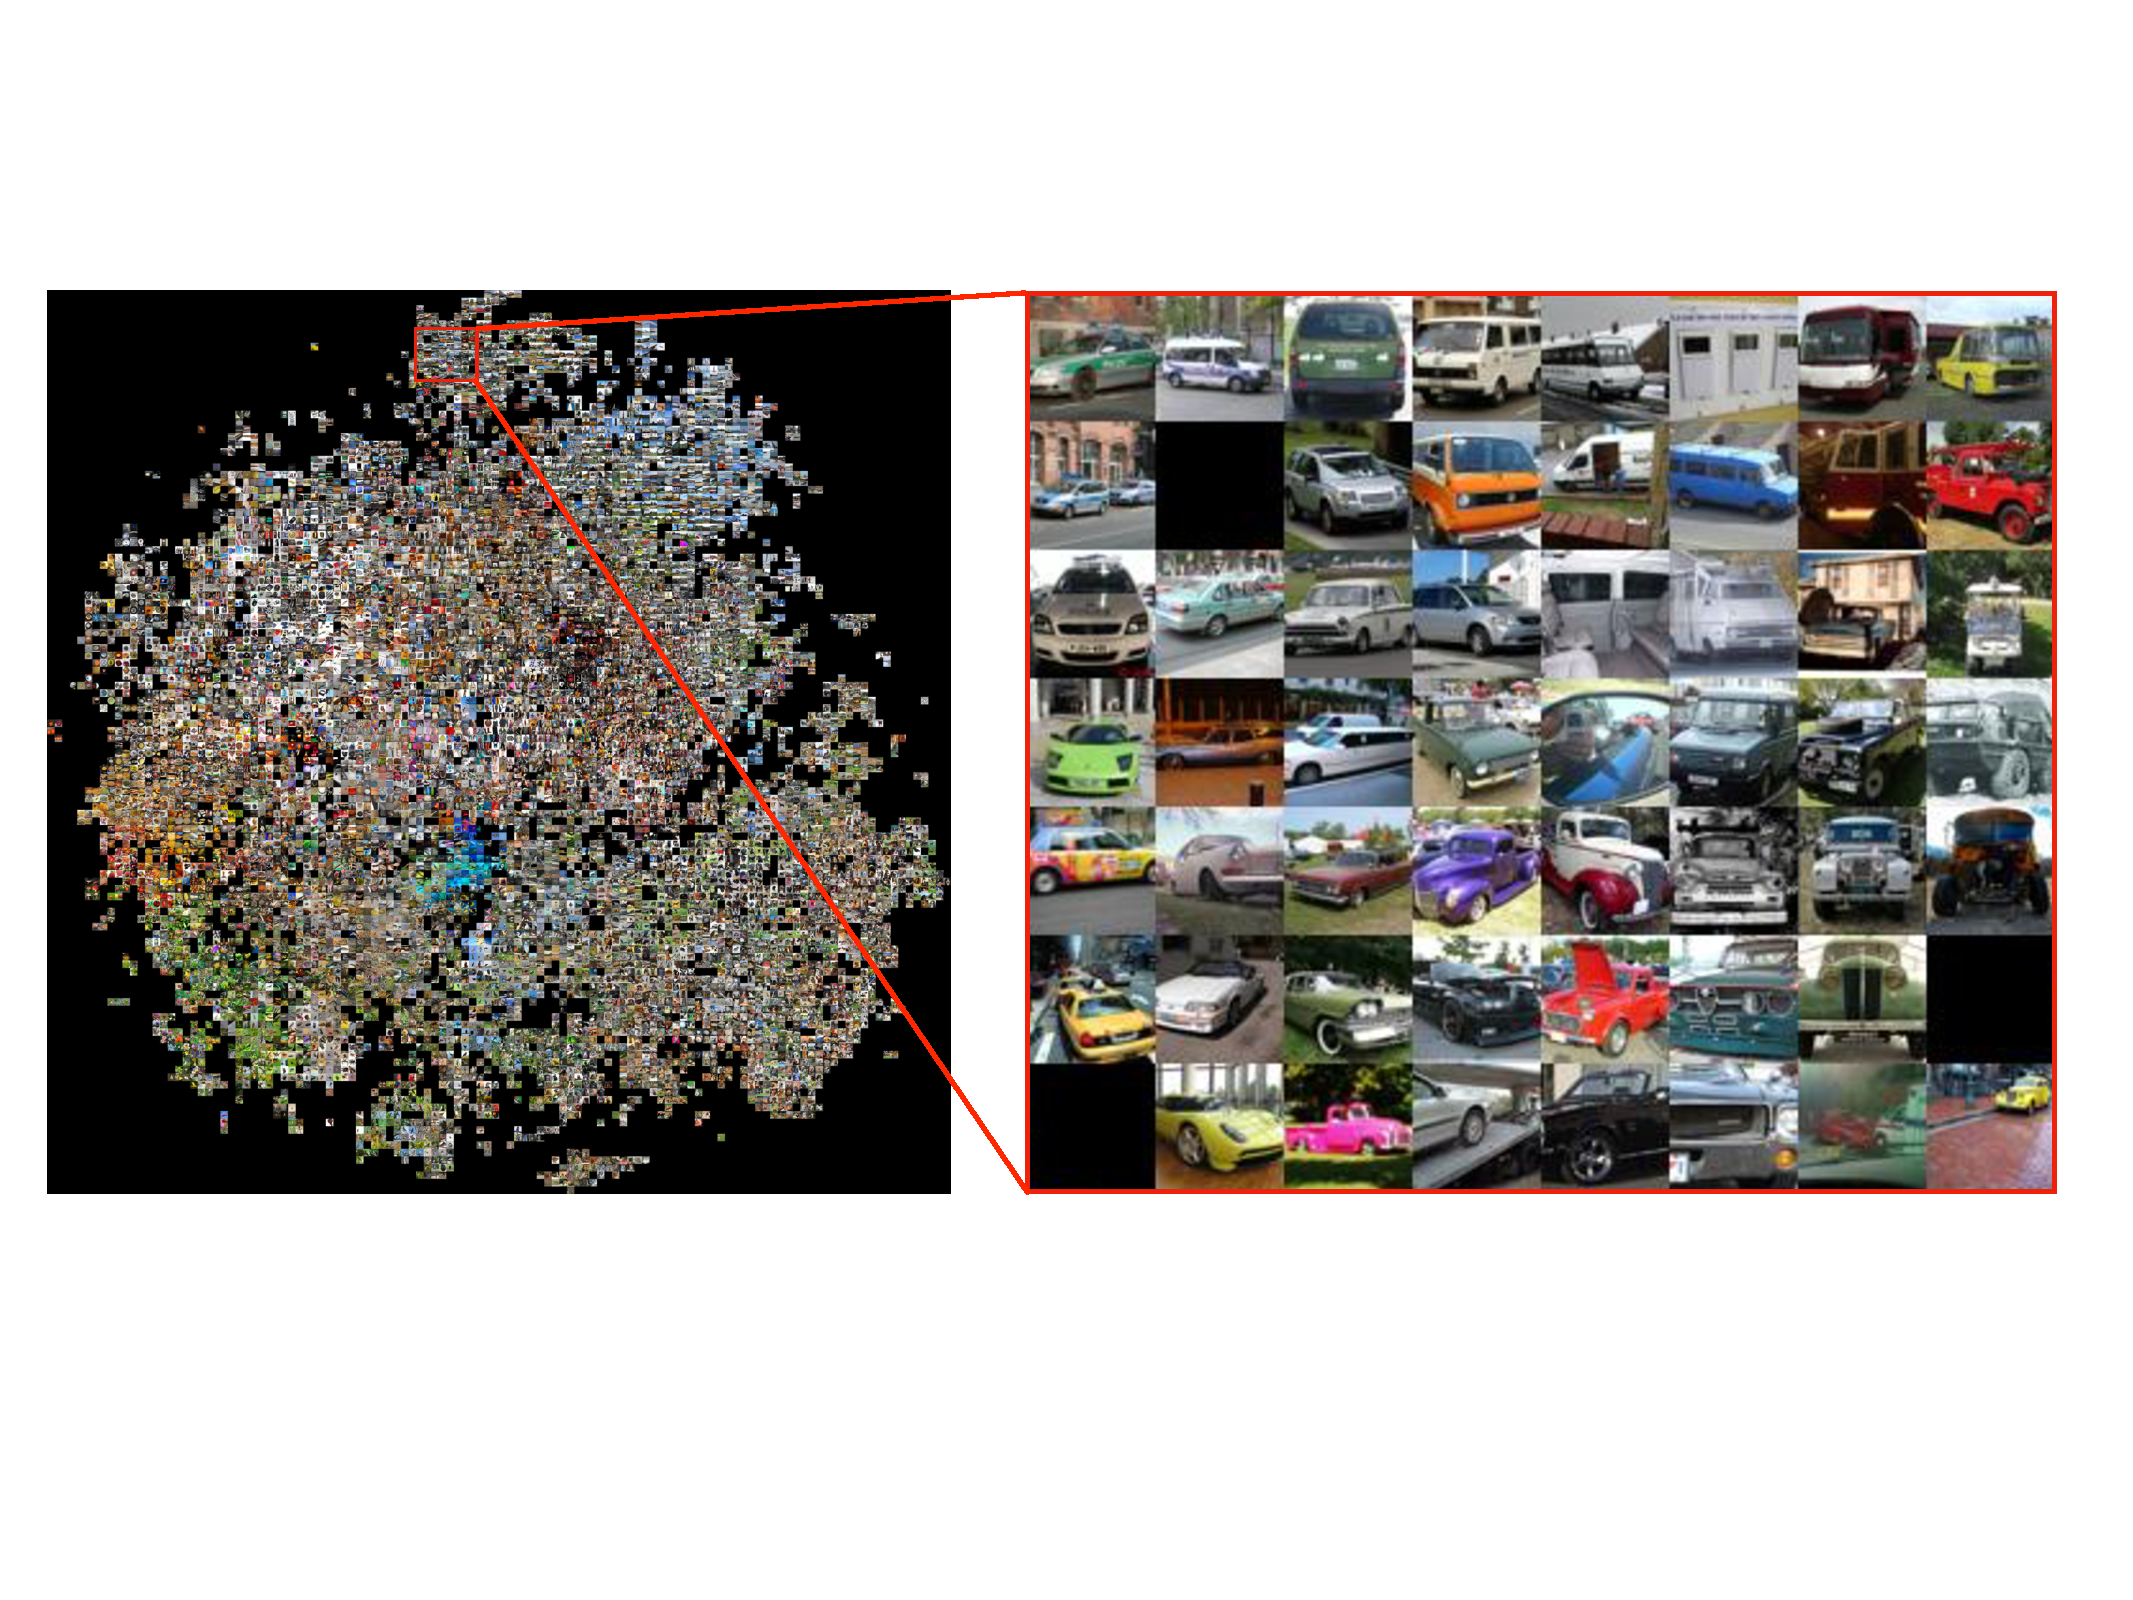
\includegraphics[width=\textwidth]{Vis_tsne_imagenet1.pdf}
%  \source{adapted from \url{https://cs.stanford.edu/people/karpathy/cnnembed/}}
\end{figure}
\end{frame}

\begin{frame}
\frametitle{t-SNE map: ImageNet}
\begin{figure}[htb]
  \centering
  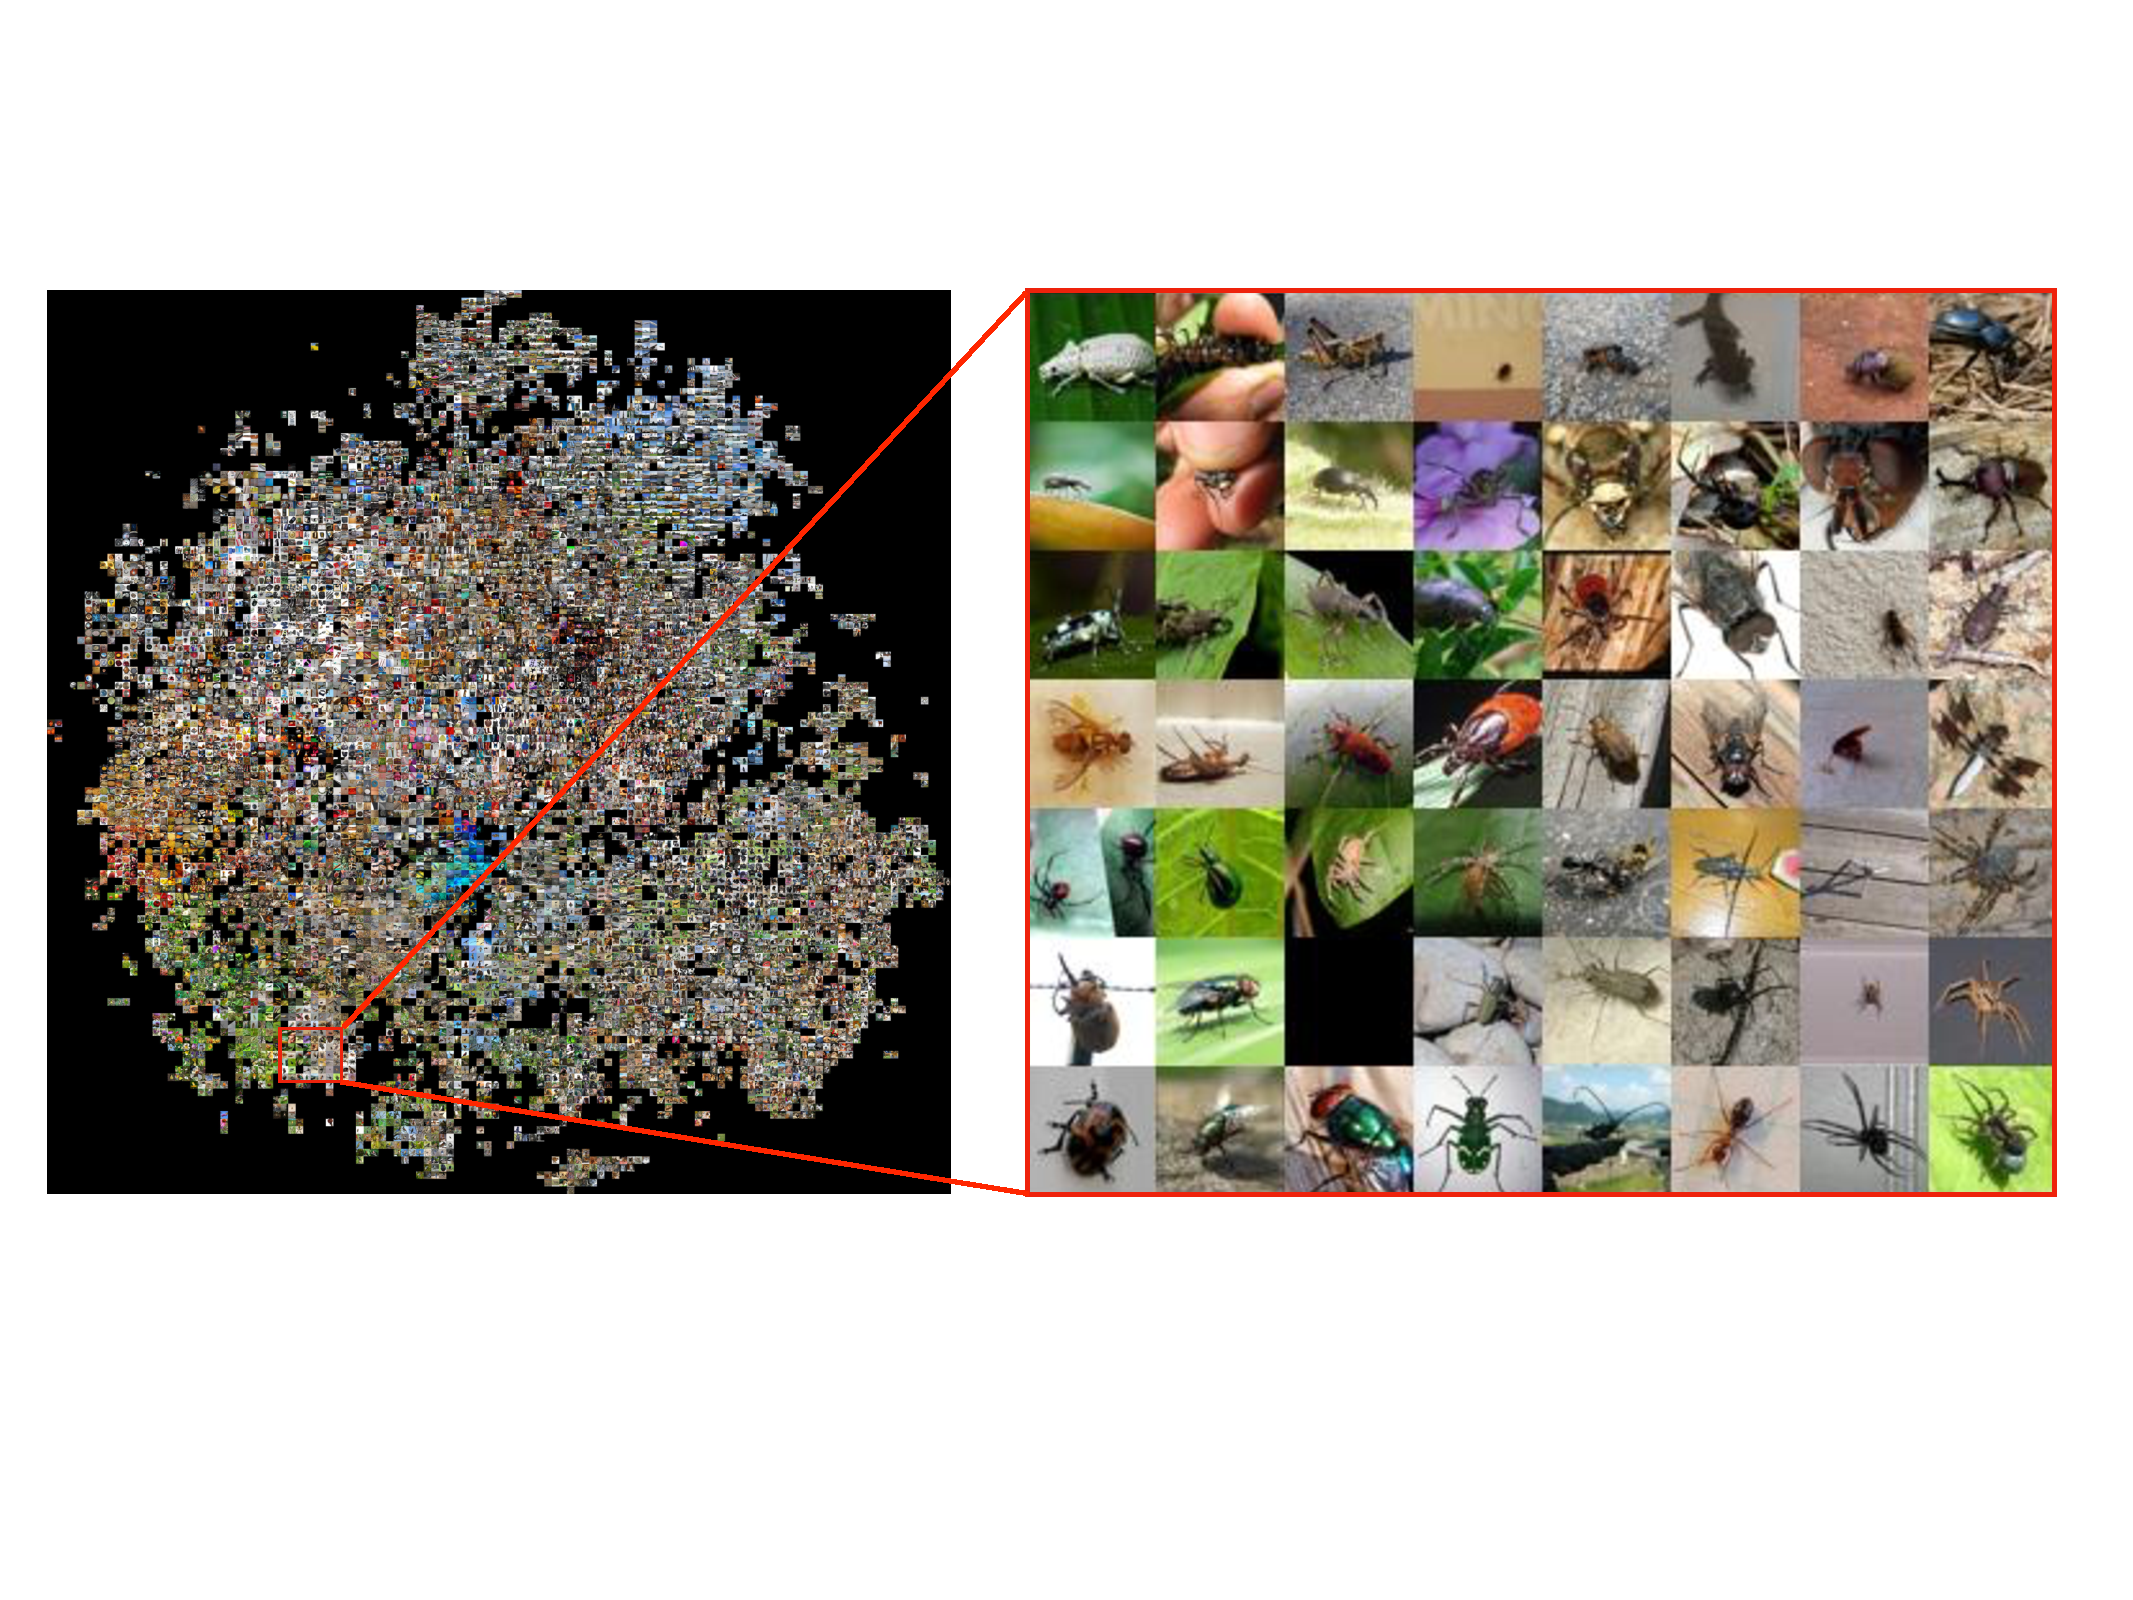
\includegraphics[width=\textwidth]{Vis_tsne_imagenet2.pdf}
%  \source{adapted from \url{https://cs.stanford.edu/people/karpathy/cnnembed/}}
\end{figure}
\end{frame}

\begin{frame}
\frametitle{t-SNE map: ImageNet}
\begin{figure}[htb]
  \centering
  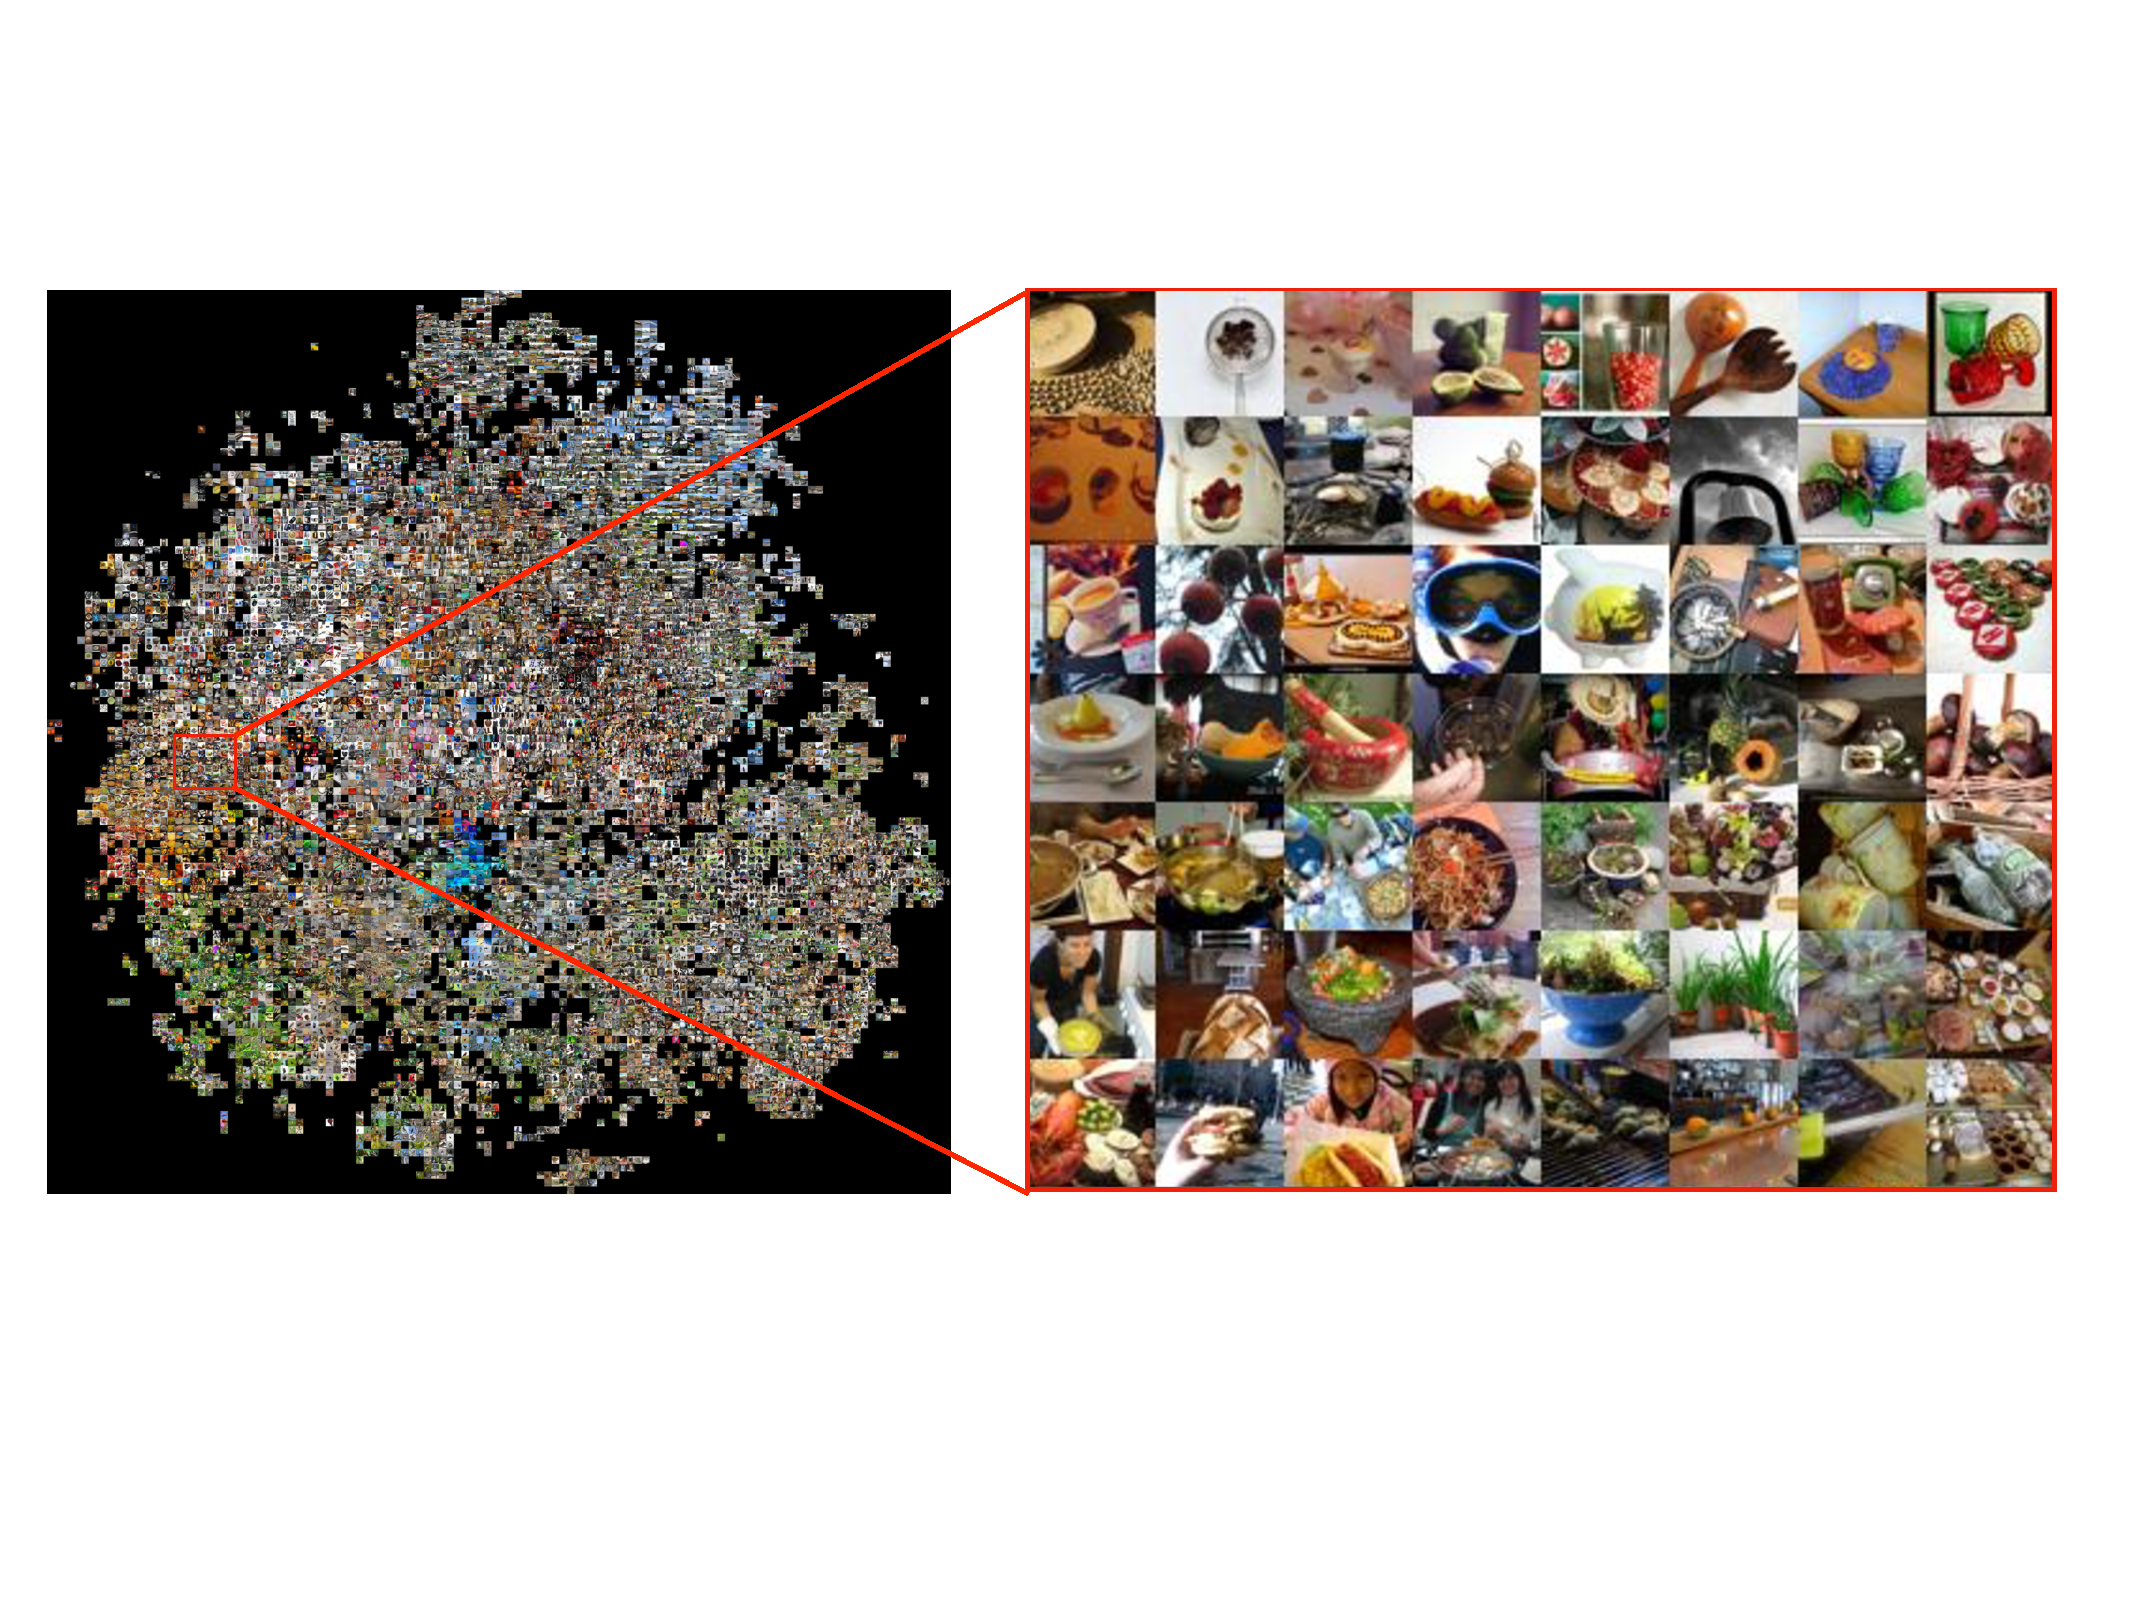
\includegraphics[width=\textwidth]{Vis_tsne_imagenet3.pdf}
%  \source{adapted from \url{https://cs.stanford.edu/people/karpathy/cnnembed/}}
\end{figure}
\end{frame}

\begin{frame}
\frametitle{Conclusion}
\begin{itemize}
	\item Méthodes de sélection par filtrage ad-hoc
	\item Méthodes de conteneur : sélection de variables pour une classification spécifique
	\item Méthodes embarquées (LASSO, ... )
	\item APC : analyse en composante principale
	\item t-SNE : méthode utilisée pour la visualisation. 
\end{itemize}
\end{frame}




\begin{frame}
  \begin{center}
    \red{\LARGE Cours 6 -- Clustering} 
  \end{center}
\end{frame}
%clustering



\begin{frame}
  \frametitle{Clustering - Motivation}
  \begin{itemize}
  	\item Etude des données non étiquetées
  	\item Analyse exploratoire
  	\item Séparation des données en sous-groupes homogènes, appelés \red{clusters}.
  	\item Visualisation
  	\item Première étape pour l'apprentissage supervisé
  \end{itemize}
\end{frame}


\begin{frame}
  \frametitle{Clustering - Exemples}
  \begin{itemize}
  	\item utilisateurs qui ont des comportements similaires 
  	\item communautés sur un réseau social
  	\item motifs récurrents dans des transactions financières
  	\item des pixels d’un même objet dans une image (segmentation d’image)
  	\item des patients dont la maladie s’explique par un même profil génétique
  \end{itemize}
\end{frame}

\begin{frame}
\frametitle{Critère de qualité 1/5}
\begin{itemize}
	\item Définition centroïde du cluster $\cset$: $\muvec_{\cset} = \frac{1}{\cset}\sum_{\xvec \in \cset}\xvec$
	\item Définition médoïde du cluster $\cset$: $\mvec_{\cset} = \argmin_{\xvec \in \cset}d(\xvec, \muvec_{\cset})$
	\item \red{Homogénéité} d'un cluster $k$: 
	\begin{equation*}
	T_k = \frac{1}{|\cset_k|} \sum_{\xvec \in \cset_k} d(\xvec, \muvec_k)
	\end{equation*}
	\item Homogénéité d'un clustering : 
	\begin{equation*}
	T = \frac1K\sum_{k=1}^{K}T_k
	\end{equation*}
\end{itemize}
\end{frame}

\begin{frame}
\frametitle{Critère de qualité 2/5}
\begin{itemize}
	\item Séparabilité des clusters $k$ et $l$ : 
	\begin{equation*}
	s_{kl} = d(\muvec_k, \muvec_l)
	\end{equation*}
	\item Séparabilité globale : 
	\begin{equation*}
	S = \frac{2}{K(K-1)}\sum_{k=1}^{K-1}\sum_{l=k+1}^{K}s_{kl}
	\end{equation*}
\end{itemize}
\end{frame}

\begin{frame}
\frametitle{Critère de qualité 3/5}
\begin{itemize}
	\item Critère de Davis-Bouldin (homogénéité et séparabilité ensemble): 
	\begin{equation*}
	D_k = \max_{l\neq k} \frac{T_k + T_l}{S_{kl}}
	\end{equation*}
	\item Critère de Davis-Bouldin pour un clustering entier : 
	\begin{equation*}
	D = \frac1K \sum_{k=1}^{K}D_k
	\end{equation*}
\end{itemize}
\end{frame}

\begin{frame}
\frametitle{Critère de qualité 4/5}
\begin{itemize}
	\item Coefficient de silhouette. On note d'abord $a(\xvec)$ comme la moyenne des distances de $\xvec$ et des autres points dans le cluster $k(\xvec)$ auquel $\xvec$ est assigné. 	
	\begin{equation*}
	a(\xvec) = \frac{1}{|\cset_{k(\xvec)}| - 1} \sum_{\uvec \in \cset_{k(\xvec)}}d(\xvec, \uvec)
	\end{equation*}
	\item La valeur $b(\xvec)$ correspond à la même expression, mais calculée pour le cluster autre que $k(\xvec)$, pour lequel la valeur est minimale: 	
	\begin{equation*}
	b(\xvec) = \min_{l\neq k(\xvec)}\frac{1}{|\cset_l|} \sum_{u \in \cset_l}d(\uvec, \xvec)
	\end{equation*}
\end{itemize}
\end{frame}

\begin{frame}
\frametitle{Critère de qualité 5/5}
\begin{itemize}
	\item Avec $a$ et $b$ définis ainsi, nous pouvons définir le coefficient de silhouette pour le point $\xvec$ : 
	\begin{equation*}
	s(\xvec) = \frac{b(\xvec)-a(\xvec) }{\max{(b(\xvec), a(\xvec))}  }
	\end{equation*}
	\item Finalement, le \red{coefficient de silhouette} pour le clustering est :
	\begin{equation*}
	s = \frac1n \sum_{i=1}^{n}s(\xvec^i)
	\end{equation*}

\end{itemize}
\end{frame}

%%%%%%%%%%%%%%%% hierarchical clustering
\begin{frame}
\frametitle{Clustering hiérarchique agglomératif}
\begin{itemize}
\item Commencer avec des points de données individuels en tant que clusters distincts.
\item Fusionner les deux clusters les plus proches.
\item Calculer la nouvelle représentation du cluster unique.
\item Répéter cela jusqu'à ce qu'il n'y ait plus rien à fusionner.
\end{itemize}
\end{frame}

\begin{frame}
\frametitle{Clustering hiérarchique divisif}
\begin{itemize}
\item Commencer avec un seul cluster.
\item Diviser le cluster en deux selon une heuristique quelconque.
\item Répéter cela jusqu'à ce qu'on ait des points individuels.
\item Ici, nous traitons uniquement des méthodes de clustering hiérarchique agglomératif (beaucoup plus répondu). 
\end{itemize}
\end{frame}

\begin{frame}
\frametitle{Éléments du clustering hiérarchique}
\begin{itemize}
\item Distance entre points
\item Une règle de fusion de clusters (fonction d'agglomeration)
\end{itemize}
\end{frame}

\begin{frame}
\frametitle{Les distances entre points}
La distance est une fonction 
\begin{equation*}
d: \mathcal{X} \times \mathcal{X} \mapsto \RR^{+} 
\end{equation*}
qui remplit les conditions suivantes : 
\begin{itemize}
\item Symmétrie : $d(a, b) = d(a, b)$
\item Séparation : $d(a, b) \Leftrightarrow a=b$
\item Inégalité triangulaire : $d(a,b) \leq d(a,c) + d(c,b)$
\end{itemize}
\end{frame}

\begin{frame}
\frametitle{Distances entre points}
\begin{itemize}
\item Distance Euclidienne: $d^2(\xvec_i, \xvec_j) = \langle \xvec_i-\xvec_j, \xvec_i-\xvec_j \rangle = \sum_k(x_{i,k}-x_{j,k})^2$
\item Distance Manhattan: $d(\xvec_i, \xvec_j) = \sum_k|x_{i,k}-x_{j,k}|$
\item Distance Euclidienne généralisée : $d^2(\xvec_i, \xvec_j) = (\xvec_i - \xvec_j)^TA(\xvec_i - \xvec_j)$ (exemple: distance Mahalanobis, avec $A=\Sigma^{-1}$)
%\item Distance basée sur la correlation : $d(\xvec_i, \xvec_j) = \frac{1}{2} - \frac{1}{2}\ro(\xvec_i, \xvec_j)$
%\item Distance cosinus : $d(\xvec_i, \xvec_j) = \frac{1}{2} - \frac{1}{2}\frac{\angle \xvec_i, \xvec_j \rangle}{\|\xvec_i\|\|\xvec_j\|} $
\end{itemize}
\end{frame}

% \item Single linkage: $d_{A,B} = \min_{(\xvec_i, x_j) \in A \times B}{d(\xvec_i, \xvec_j)}$
% \item Complete linkage: $d_{A,B} = \max_{(\xvec_i, \xvec_j) \in A \times B}{d(\xvec_i, \xvec_j)}$
% \item Average linkage: $d_{A,B} = \frac{1}{N_AN_B} \sum_{(\xvec_i, \xvec_j) \in A \times B} d(\xvec_i, \xvec_j)$
% \item Centroid: $d_{A,B} = d(\mu_A, \mu_B)$ with $\mu_A$, $\mu_B$ the average of $\xvec$ in $A$ and $B$ respectively.  
% \item Ward: $d_{A,B} = \frac{N_AN_B}{N_A+N_B}\|\mu_A - \mu_B\|^2$ with $\mu_A$, $\mu_B$ the average of $\xvec$ in $A$ and $B$ respectively. The ward method chooses the cluster fusion producing the smallest increase in variance. 



\begin{frame}
\frametitle{Fonctions d'agglomération}
\begin{figure}[htb]
  \centering
  \includegraphics[width=.8\textwidth]{SingleLinkage}
  \caption{Single Linkage}
\end{figure}
Single Linkage: 
\begin{equation*}
d_{A,B} = \min_{(\xvec_i,\xvec_j) \in A \times B}{d(\xvec_i, \xvec_j)}
\end{equation*}

\end{frame}


\begin{frame}
\frametitle{Fonctions d'agglomération}
\begin{figure}[htb]
  \centering
  \includegraphics[width=.8\textwidth]{CompleteLinkage}
  \caption{Complete Linkage}
\end{figure}
Complete linkage: $d_{A,B} = \max_{(\xvec_i, \xvec_j) \in A \times B}{d(\xvec_i, \xvec_j)}$
\end{frame}


\begin{frame}
\frametitle{Fonctions d'agglomération}

\begin{figure}[htb]
  \centering
  \includegraphics[width=.8\textwidth]{AverageLinkage2}
  \caption{Average Linkage}
\end{figure}
Average linkage: $d_{A,B} = \frac{1}{N_AN_B} \sum_{(\xvec_i, \xvec_j) \in A \times B} d(\xvec_i, \xvec_j)$
\end{frame}



\begin{frame}
\frametitle{Fonctions d'agglomération}

\begin{figure}[htb]
  \centering
  \includegraphics[width=.8\textwidth]{CentroidLinkage}
  \caption{Centroid Linkage}
\end{figure}
Centroid: $d_{A,B} = d(\mu_A, \mu_B)$ with $\mu_A$, $\mu_B$ the average of $\xvec$ in $A$ and $B$ respectively.  
\end{frame}


\begin{frame}
\frametitle{Fonctions d'agglomération}
\begin{figure}[htb]
  \centering
  \includegraphics[width=.8\textwidth]{WardLinkage}
  \caption{Ward Linkage}
\end{figure}
Ward: $d_{A,B} = \frac{N_AN_B}{N_A+N_B}\|\overrightarrow{\mu}_A - \overrightarrow{\mu}_B\|^2$
$\overrightarrow{\mu}_A$, $\overrightarrow{\mu}_B$ sont les moyennes de $\xvec$ dans $A$, $B$. La méthode de Ward choisit la fusion qui produit la plus petite augmentation de la variance intra-cluster. 
\end{frame}

\begin{frame}
\frametitle{Clustering hiérarchique : exemple}
\begin{figure}[htb]
  \centering
  \includegraphics[height=0.7\textheight]{HierarchicalClustering_Example}
  \caption{Exemple: clustering hiérarchique sur des données d'expression génétique dans le cancer du poumon (colonnes : tissue, lignes : gènes)}
\end{figure}
\end{frame}



%%%%%%%%%%%%%%%% k-means
\begin{frame}
\frametitle{Méthode des k-moyennes}
\begin{itemize}
	\item On fixe un nombre $K$ de clusters. 
	\item On essaie de trouver une affectation des points $\xvec_i$ aux clusters afin de minimiser l'intra-cluster variance : 
	\begin{equation*}
	\argmin_{\cset_1, \cset_2, \ldots, \cset_K} \sum_{k=1}^K \sum_{\xvec \in \cset_k} \ltwonorm{\xvec - \muvec}^2
	\end{equation*}
\end{itemize}
\end{frame}

\begin{frame}
\frametitle{Méthode des k-moyennes : algorithme de Lloyd}
\begin{enumerate}
	\item Initialisation : choisir les $\muvec_1, \muvec_2, \ldots, \muvec_K$ parmi les points $\xvec$. 
	\item Affecter chaque observation $\xvec \in \dset$ au centroïde dont elle est le plus proche :
	\begin{equation*}
		k(\xvec^i) = \argmin_{k=1, \ldots, K}\ltwonorm{\xvec^i - \muvec_k}^2
	\end{equation*}
	\item Recalculer les centroïdes $\muvec_k$. 
	\item Répéter jusqu'à ce que les affectations ne changent plus. 
\end{enumerate}
\end{frame}

\begin{frame}
\frametitle{Algorithme de Lloyd - limitations}
\begin{itemize}
\item L'algorithme de Lloyd converge très rapidement. 
\item \blue{Problème} : l'algorithme est glouton (greedy) et peut rester dans un minimum local. \blue{Solution} : répéter l'algorithme $t$ fois et prendre la solution avec la meilleure intra-cluster variance. 
\item \blue{Problème} : dépendance de l'initialisation. \blue{Solution} : placer les centres avec dispersion maximale.
\item \blue{Problème} : les clusters sont nécessairement convexes. \blue{Solution} : l'astuce de noyau peut s'appliquer ici aussi. 
\end{itemize}
\end{frame}

\begin{frame}
\frametitle{k-moyennes: avantages et inconvénients}
  \begin{itemize}
  	\item Avantages : 
  	\begin{itemize}
  		\item rapide
  		\item optimisation globale
  	\end{itemize}
  	\item Inconvénients : 
  	\begin{itemize}
  		\item il faut déterminer $K$
  		\item Problème non-convexe
  		\item Forme convexe des clusters
  	\end{itemize}
  	\item L'algorithme des k-moyennes est l'un des plus répandus en apprentissage non-supervisé. 
  \end{itemize}
\end{frame}

\begin{frame}
\frametitle{DBSCAN - Motivation}
\begin{figure}[htb]
  \centering
  \includegraphics[width=.8\textwidth]{dbscan_motivation}
  \caption{Échec d'algorithmes sur le problème de cercles concentriques}
\end{figure}
\red{Idée : utiliser les densités locales}
\end{frame}



\begin{frame}
\frametitle{DBSCAN - Algorithme}
\begin{itemize}
	\item On définit : 
	\begin{itemize}
		\item Un voisinage $\nset_{\epsilon}$ (boule autour de chaque point, avec rayon $\epsilon$)
		\item Un nombre minimal de voisins $n_{min}$ dans le voisinage. 
	\end{itemize}
	\item On considère chaque point comme aberrant (outlier), s'il ne remplit pas le critère du nombre minimal. 
	\item On itère sur les points $\xvec \in \dset$, et on ajoute tous les points qui sont atteignables de $\xvec$ avec un chemin qui ne requiert pas de distance entre points plus grande que $\epsilon$. 
\end{itemize}
\end{frame}

\begin{frame}
\frametitle{DBSCAN - chemin / résultats}
\begin{figure}[htb]
  \centering
  \includegraphics[width=.8\textwidth]{dbscan}
\end{figure}
\begin{itemize}
	\item À gauche, on voit le chemin qui est utilisé dans l'algorithme. 
\end{itemize}
\end{frame}

\begin{frame}
\frametitle{DBSCAN : avantages et inconvénients}
  \begin{itemize}
  	\item Avantages : 
  	\begin{itemize}
  		\item n'impose pas de forme particulière
  		\item simple, pas de définition du nombre de clusters
  		\item robustesse aux données aberrantes
  	\end{itemize}
  	\item Inconvénients : 
  	\begin{itemize}
  		\item ne sait pas gérer des écarts
  		\item peu de résultats théoriques
  		\item pas applicable en très haute dimension (à cause de la définition de $\nset_{\epsilon}$)
  	\end{itemize}
  \end{itemize}
\end{frame}


\begin{frame}
\frametitle{Conclusion (clustering)}
\begin{itemize}
	\item Le clustering, ou partitionnement de données, cherche à identifier des classes sans utiliser d’étiquettes
	\item La qualité d’une partition peut s’évaluer sur des critères de séparabilité et d’homogénéité
	\item k-moyennes: Il permet de trouver efficacement K clusters convexes.
	\item DBSCAN : détection des formes non-convexes (en basse dimension). 
\end{itemize}
\end{frame}

\begin{frame}
\frametitle{Conclusion générale - avant de commencer}
\begin{itemize}
\item Spécification du problème : 
\begin{itemize}
	\item supervisé ou non-supervisé ? 
	\item régression ou classification ? 
\end{itemize}
\item Quantification pour la mise en place:
\begin{itemize}
	\item combien de descripteurs ($p$) ? 
	\item combien d'échantillons annotés ($n$) ? 
	\item combien d'échantillons non-annotés ?
\end{itemize}
\end{itemize}
\end{frame}

\begin{frame}
\frametitle{Conclusion générale - avant de commencer}
\begin{itemize}
	\item Exigences supplémentaires : 
	\begin{itemize}
		\item interprétabilité des modèles
		\item robustesse 
		\item compromis sensibilité / précision
		\item biais et perturbations potentiels
	\end{itemize}
\end{itemize}
\end{frame}

\begin{frame}
\frametitle{Conclusion générale - méthodes non-supervisées}
\begin{itemize}
	\item Exploration graphique des données : 
	\begin{itemize}
		\item Réduction de dimensions (ACP, t-SNE)
		\item Clustering pour trouver des groupes
	\end{itemize}
	\item Le but est comprendre les distributions des données et éventuellement d'identifier des groupes. 
	\item Visualisation joue souvent un rôle clé pendant cette phase exploratoire.
\end{itemize}
\end{frame}

\begin{frame}
\frametitle{Conclusion générale - problèmes supervisés}
\begin{itemize}
	\item Si $n \gg p$ : 
	\begin{itemize}
		\item des méthodes classiques comme la $LDA$ ou la régression logistique peuvent s'appliquer. 
		\item Problème potentiel : corrélation des descripteurs. Solution possible : sélectionner les descripteurs, ou bien appliquer une $ACP$. 
		\item Tester l'effet d'une régularisation. 
	\end{itemize}
	\item Si $p > n$ (et même si $p \gg n$): 
	\begin{itemize}
		\item les $SVM$ ou les $RF$ sont préférables. 
		\item la régularisation se fait avec la norme $L_2$ des paramètres pour les $SVM$ et par ensembling pour les $RF$. 
	\end{itemize}
\end{itemize}
\end{frame}

% \begin{frame}
% \frametitle{Conclusion générale - problèmes supervisés}
% \begin{itemize}
% 	\item Fixer les hyper-paramètres par validation croisée. 
% 	\item Évaluation de performance sur un jeu de données pas utilisé pour l’entraînement ou la sélection de modèles.
% 	\item Tests supplémentaires concernant la robustesse, le temps de calcul, etc. 
% \end{itemize}
% \end{frame}



% \begin{frame}
% \frametitle{Conclusion générale}
% \begin{itemize}
% 	\item 
% 	\item La qualité d’une partition peut s’évaluer sur des critères de séparabilité et d’homogénéité
% %— Le clustering hiérarchique partitionne les données de manière itérative. Son résultat peut être vi- sualisé sur un dendrogramme.
% 	\item k-moyennes: Il permet de trouver efficacement K clusters convexes.
% %— Laversionànoyaudelaméthodedesk-moyennespermetdel’appliquerpourdécouvrirdesclusters non convexes.
% 	\item DBSCAN : détection des formes non-convexes (en basse dimension). 
% %— Le clustering par densité permet d’identifier des régions denses du jeu de données, c’est-à-dire des observations qui peuvent former un ensemble non convexe mais qui sont proches les unes des autres.
% \end{itemize}
% \end{frame}




\begin{frame}
  \frametitle{Références / page pub}
  \begin{itemize}
  \item \black{Introduction au Machine Learning}, Chloé-Agathe Azencott, Dunod InfoSup \\
    Version électronique (PDF) sans exercices disponible gratuitement sur  \textcolor{MyBlue}{\href{http://cazencott.info/dotclear/public/lectures/IntroML_Azencott.pdf}{http://cazencott.info [lien cliquable]}}\\
    (nouvelle édition en préparation)
  \item \black{Le Machine Learning avec scikit-learn}, Aurélien Géron, Dunod
    InfoSup
  \item Textes et vidéos sur \blue{OpenClassrooms :} \\
    {\footnotesize Textes accessibles librement ; vidéos accessibles avec un compte gratuit.}
    \begin{itemize} 
    \item \textcolor{MyBlue}{\href{https://openclassrooms.com/fr/paths/148-ingenieur-machine-learning\#path-tabs}{Parcours Ingénieur Machine Learning [lien cliquable]}}
     \item \textcolor{MyBlue}{\href{https://openclassrooms.com/fr/courses/6417031-objectif-ia-initiez-vous-a-lintelligence-artificielle}{Objectif IA (grand public)  [lien cliquable]}}
    \end{itemize}
  \end{itemize}
\end{frame}

\begin{frame}
  \frametitle{Ressources complémentaires}
  \begin{itemize}
  \item \blue{Sources de jeux de données}
    \begin{itemize}
    \item Kaggle \href{https://www.kaggle.com/}{[lien cliquable]}
    \item Le module \texttt{datasets} de \texttt{scikit-learn} \textcolor{MyBlue}{\href{https://sklearn.org/datasets/index.html}{[lien cliquable]}}
    \item Le UCI Machine Learning Repository \textcolor{MyBlue}{\href{https://archive.ics.uci.edu/ml/index.php}{[lien cliquable]}}
    \end{itemize}
  \item \blue{MOOC scikit-learn } \textcolor{MyBlue}{\href{https://inria.github.io/scikit-learn-mooc/}{[lien cliquable]}}
  \end{itemize}
\end{frame}


% \begin{frame}
%   \begin{center}
%     \red{\LARGE Cours 5 -- Réduction de dimension} 
%   \end{center}
% \end{frame}
% %% dimred

\begin{frame}
  \frametitle{Réduction de dimensions - Problème}
  \begin{itemize}
  \item Grand nombre $p$ de variables (centaines ou milliers de variables).
  \item Si $n$ est grand, on parle de \red{big data}.   
  \item Si $p$ est grand par rapport à $n$, on parle de \red{fat data}. 
  \item Réduction de dimensions : trouver pour une matrice de données $X\in \RR^{n\times p}$ une représentation $X \in \RR^{n\times m}$, avec $p\gg m$. 
  \end{itemize}
\end{frame}

\begin{frame}
  \frametitle{Réduction de dimensions - Motivation}
  \begin{itemize}
  \item Visualisation / exploration : une étape importante
  \item Identifier des artefacts
  \item Réduction du coût computationnel
  \item Moins de descripteurs pour de meilleurs algorithmes de prédiction : 
  \begin{itemize}
  	\item moins de paramètres à estimer
  	\item moins de bruit
  	\item moins de dimensions peu informatives
  	\item éviter le fléau de la dimensionalité
  \end{itemize}
  \end{itemize}
\end{frame}

\begin{frame}
  \frametitle{Réduction de dimensions - deux stratégies}
  \begin{itemize}
  	\item \red{Sélection de variables} : éliminer les variables peu utiles
  	\item \red{Extraction de variables} : créer $m$ nouvelles variables à partir des $p$ variables
  \end{itemize}
\end{frame}

\begin{frame}
  \frametitle{Méthode de filtrage}
  \begin{itemize}
  	\item Filtrage non-supervisé (exemple : enlever des variables corrélées )
  	\item Filtrage supervisé : enlever des variables qui ne sont pas statistiquement associées à la variable de sortie
  \end{itemize}
\end{frame}

\begin{frame}
  \frametitle{Méthode de filtrage - limitations}
	\begin{figure}[htb]
	  \centering
	  \includegraphics[width=.6\textwidth]{guyon.pdf}
	%  \source{adapted from \url{https://cs.stanford.edu/people/karpathy/cnnembed/}}
	\end{figure}
  	Des variables corrélées et non-significatives peuvent tout de même être utiles (dans le contexte d'autres variables).
\end{frame}

\begin{frame}
  \frametitle{Méthode de conteneur}
  \begin{itemize}
  	\item Méthode supervisée de sélection de variables. 
  	\item Liée à une méthode de classification : on juge la qualité de la variable par rapport à la performance de classification.
  	\item 2 stratégies : 
  	\begin{itemize}
  		\item \red{Méthode ascendante (forward selection)}: successivement ajouter des variables
  		\item \red{Méthode descendante (backward selection)}: successivement enlever des variables
  	\end{itemize}
  \end{itemize}
\end{frame}

\begin{frame}
  \frametitle{Méthode ascendante}
  \begin{itemize}
  	\item On commence avec un ensemble de variables vide $\fcal = \emptyset$
  	\item A chaque étape, on ajoute la variable qui apporte le meilleur gain en performance de classification.
  	\item On arrête, quand la performance ne s'améliore plus. 
  \end{itemize}
\end{frame}

\begin{frame}
  \frametitle{Méthode descendante}
  \begin{itemize}
  	\item On commence avec l'ensemble de toutes les variables $\fcal$
  	\item A chaque étape, on enlève la variable sans laquelle on obtient la meilleure performance de classification.
  	\item On arrête, quand la performance ne s'améliore plus. 
  \end{itemize}
\end{frame}

\begin{frame}
  \frametitle{Méthode de conteneur - limitations}
  \begin{itemize}
  	\item L'ensemble de variables identifiés dépend du classifieur utilisé (il ne s'agit pas d'un critère général). 
  	\item Méthode gloutonne (greedy method): aucune garantie d'optimalité. 
  \end{itemize}
\end{frame}

\begin{frame}
  \frametitle{Méthodes embarquées}
  \begin{itemize}
  	\item Méthodes de classification avec un mécanisme de sélection de variables
  	\item Exemple : l'utilisation de la norme $L_1$ (valeur absolue).  
  	\item Pour rappel : 
  \end{itemize}
  \begin{center}
    \includegraphics[width=.6\textwidth]{figures/l1reg_geom}  
  \end{center}
\end{frame}

\begin{frame}
  \frametitle{Analyse en composantes principales}
  \begin{itemize}
  	\item Analyse en composantes principales (ACP) (principal component analysis, PCA)
  	\item Méthode non-supervisée (aucune étiquette est utilisée)
  	\item Expression de $X\in \RR^{n\times p}$ dans une base orthonormée, par une transformation linéaire orthogonale.
  	\item Maximisation de la variance.
%  	\item Premier axe : projection de $X$ avec la plus grande variance
%  	\item Deuxième axe : projection de $X$ avec la plus grande variance, orthogonale à la première. 
%  	\item $\ldots$
  \end{itemize}
\end{frame}

\begin{frame}
  \frametitle{Extraction de variables - ACP}
	\begin{figure}[htb]
	  \centering
	  \includegraphics[width=.8\textwidth]{pca.pdf}
	%  \source{adapted from \url{https://cs.stanford.edu/people/karpathy/cnnembed/}}
	\end{figure}
\end{frame}

\begin{frame}
\frametitle{ACP: Méthode 1/3}
  \begin{itemize}
  	\item Première étape : centrer les colonnes de $X \in \RR^{n \times p}$: 
 \begin{equation*}
 x^i_j = \frac{x_j^i - \overline{x}_j}{\sqrt{\frac{1}{n}\sum_{l=1}^n(x_j^l - \overline{x}_j)^2}} 
 \end{equation*}
 	\item La matrice de covariance est donc : $\Sigma = \frac1n X^TX$ 
 	\item On cherche maintenant une direction $\wvec$, pour laquelle la projection de $X$ sur cette direction a une variance maximale. 
 	\item On peut montrer que cette variance maximale est la plus grande valeur propre de $\Sigma$, et que la direction est le vecteur propre correspondant. 
  \end{itemize}
\end{frame}

\begin{frame}
\frametitle{ACP: Méthode 2/3}
  \begin{itemize}
  	\item Si on ordonne les valeurs propres de $\Sigma$ selon leurs tailles, on obtient les composantes principales $cp_2, cp_3, \ldots$ qui remplissent les critères suivants : 
  	\begin{itemize}
  		\item Chaque $cp_i$ est orthogonal à toutes les autres composantes.
  		\item La variance de la projection de $X$ sur $cp_i$ est identique à la valeur propre $i$. 
  	\end{itemize}
  	\item Nous en déduisons : 
  	\begin{itemize}
  		\item Les projections de $X$ sur les composantes principales sont décorrélées. 
  		\item Les composantes principales $cp_i$ contiennent de moins en moins d'information (avec $i$ croissant). 
  	\end{itemize}
  \end{itemize}
\end{frame}

\begin{frame}
\frametitle{ACP: Méthode 3/3}
  \begin{itemize}
  	\item L'ACP nous donne donc une transformation avec : des variables décorrélées, et ordonnées selon l'importance. 
  	\item Typiquement, on choisit un nombre $m$ de composantes principales. Le critère pour $m$ est la variance "expliquée" par le modèle. 
  	\item On peut aussi choisir $m=2$ ou $m=3$ pour la visualisation par exemple.   
  \end{itemize}
\end{frame}

\begin{frame}
\frametitle{ACP: avantages et inconvénients}
  \begin{itemize}
  	\item Avantages : 
  	\begin{itemize}
  		\item non-supervisé
  		\item projections décorrélées 
  		\item simple, méthode linéaire
  	\end{itemize}
  	\item Inconvénients : 
  	\begin{itemize}
  		\item la variance maximale n'est pas identique avec le contenu d'information
  		\item en pratique, les structures locales ne sont pas nécessairement bien préservées 
  	\end{itemize}
  \end{itemize}
\end{frame}

\begin{frame}
\frametitle{t-SNE 1/3}
\begin{itemize}
%	\item Many low dimensional representations: PCA, ICA, $\ldots$
	\item Objectif : représentation des données en basse dimension en respectant les relations locales
	\item Une technique relativement récente  \emph{t-Distributed Stochastic Neighbor Embedding (t-SNE)} (2008)
	\item $\{\xvec_i\}_{0\leq i < N}$ sont les représentations, avec $\xvec \in \RR^p$. 
	\item On définit la probabilité que $x_j$ est voisin de $x_i$, sous condition que la probabilité peut être modélisée par une Gaussienne, centrée dans $x_i$:  
	\begin{equation}
	p_{j|i} = \frac{\exp{\left(-\frac{\|\xvec_i - \xvec_j\|^2}{2 \sigma_i^2}\right)}}{\sum_{k\neq i} \exp{\left(-\frac{\|\xvec_i - \xvec_k\|^2}{2 \sigma_i^2}\right)} }
	\end{equation}
	Le paramètre $\sigma_i$ varie avec l'échantillon $x_i$. 
\end{itemize}
\end{frame}


\begin{frame}
\frametitle{t-SNE 2/3}
\begin{itemize}
	\item On souhaite assigner aux vecteurs $\{\xvec_i\}$ des représentations $\{\widetilde{\xvec_i}\}$ tout en préservant les probabilités de voisinages $q_{j|i}$: 
	\begin{equation*}
	q_{j|i} = \frac{\exp{\left(-\|\widetilde{\xvec_i} - \widetilde{\xvec_j}\|^2\right)}}{\sum_{k\neq i} \exp{\left(-\|\widetilde{\xvec_i} - \widetilde{\xvec_k}\|^2\right)} }
	\end{equation*}
	\item Cela peut être fait par la minimisation de la divergence Kulback-Leibler entre les distributions $P_i$ (distribution de $p_{j|i}$) et $Q_i$ (distribution de $q_{j|i}$): 
	\begin{equation}
		C = \sum_i KL(P_i\|Q_i) = \sum_i \sum_j p_{j|i}\log{\frac{p_{j|i}}{q_{j|i}}}
	\end{equation}
	\item Si $\xvec_i$ and $\xvec_j$ sont proches dans l'espace originale, l'algorithme va essayer de pousser $q_{j|i}$ vers $p_{j|i}$ (pour que le ratio soit 1). 
	\item Si $\xvec_i$ et $\xvec_j$ sont loin dans l'espace d'origine, il n'est pas garanti qu'ils le soient dans l'espace à basse dimension. 
\end{itemize}
\end{frame}

\begin{frame}
\frametitle{t-SNE 3/3}
\begin{itemize}
	\item Les paramètres $\sigma_i$ sont déterminés par l'algorithme
	\item Ils varient selon la densité de voisins, de façon à ce que pour chaque $\xvec_i$ nous avons à peu près le même nombre de voisins. 
	\item L'utilisateur choisit le paramètre \textit{perplexity} qui mesure le nombre effectif de voisins. 
	\item Le problème se réduit à la solution d'un problème d'optimisation $\min_{\widetilde{\xvec_i}} C$ avec la méthode du gradient.
\end{itemize}
\end{frame}

\begin{frame}
\frametitle{t-SNE: avantages et inconvénients}
  \begin{itemize}
  	\item Avantages : 
  	\begin{itemize}
  		\item conserve les structures locales
  		\item permet d'identifier des cluster potentiels. 
  	\end{itemize}
  	\item Inconvénients : 
  	\begin{itemize}
  		\item pas de transformation : la minimisation est faite pour une ensemble de données et ne peut s'appliquer à de nouvelles données. 
  		\item Distorsion dans les longues distances. 
  	\end{itemize}
  \end{itemize}
\end{frame}

\begin{frame}
\frametitle{t-SNE map: exemple}
\begin{figure}[htb]
  \centering
  \includegraphics[width=.8\textwidth]{Vis_tsne.png}
  \caption{patterns de localisation d'ARN dans la cellule}
\end{figure}
\end{frame}


\begin{frame}
\frametitle{t-SNE map: ImageNet}
\begin{figure}[htb]
  \centering
  \includegraphics[width=\textwidth]{Vis_tsne_imagenet1.pdf}
%  \source{adapted from \url{https://cs.stanford.edu/people/karpathy/cnnembed/}}
\end{figure}
\end{frame}

\begin{frame}
\frametitle{t-SNE map: ImageNet}
\begin{figure}[htb]
  \centering
  \includegraphics[width=\textwidth]{Vis_tsne_imagenet2.pdf}
%  \source{adapted from \url{https://cs.stanford.edu/people/karpathy/cnnembed/}}
\end{figure}
\end{frame}

\begin{frame}
\frametitle{t-SNE map: ImageNet}
\begin{figure}[htb]
  \centering
  \includegraphics[width=\textwidth]{Vis_tsne_imagenet3.pdf}
%  \source{adapted from \url{https://cs.stanford.edu/people/karpathy/cnnembed/}}
\end{figure}
\end{frame}

\begin{frame}
\frametitle{Conclusion}
\begin{itemize}
	\item Méthodes de sélection par filtrage ad-hoc
	\item Méthodes de conteneur : sélection de variables pour une classification spécifique
	\item Méthodes embarquées (LASSO, ... )
	\item APC : analyse en composante principale
	\item t-SNE : méthode utilisée pour la visualisation. 
\end{itemize}
\end{frame}









\end{document}

%%% Local Variables:
%%% mode: latex
%%% TeX-master: t
%%% End:
